%  LaTeX support: latex@mdpi.com 
%  For support, please attach all files needed for compiling as well as the log file, and specify your operating system, LaTeX version, and LaTeX editor.

%=================================================================
\documentclass[aipa,article,submit,pdftex,moreauthors]{Definitions/mdpi} 
%\documentclass[preprints,article,submit,pdftex,moreauthors]{Definitions/mdpi} 
% For posting an early version of this manuscript as a preprint, you may use "preprints" as the journal. Changing "submit" to "accept" before posting will remove line numbers.

% Below journals will use APA reference format:
% admsci, aieduc, behavsci, businesses, econometrics, economies, education, ejihpe, famsci, games, humans, ijcs, ijfs, journalmedia, jrfm, languages, psycholint, publications, tourismhosp, youth

% Below journals will use Chicago reference format:
% arts, genealogy, histories, humanities, jintelligence, laws, literature, religions, risks, socsci

%--------------------
% Class Options:
%--------------------
%----------
% journal
%----------
% Choose between the following MDPI journals:
% accountaudit, acoustics, actuators, addictions, adhesives, admsci, adolescents, aerobiology, aerospace, agriculture, agriengineering, agrochemicals, agronomy, ai, air, algorithms, allergies, alloys, amh, analytica, analytics, anatomia, anesthres, animals, antibiotics, antibodies, antioxidants, applbiosci, appliedchem, appliedmath, appliedphys, applmech, applmicrobiol, applnano, applsci, aquacj, architecture, arm, arthropoda, arts, asc, asi, astronomy, atmosphere, atoms, audiolres, automation, axioms, bacteria, batteries, bdcc, behavsci, beverages, biochem, bioengineering, biologics, biology, biomass, biomechanics, biomed, biomedicines, biomedinformatics, biomimetics, biomolecules, biophysica, biosensors, biosphere, biotech, birds, blockchains, bloods, blsf, brainsci, breath, buildings, businesses, cancers, carbon, cardiogenetics, catalysts, cells, ceramics, challenges, chemengineering, chemistry, chemosensors, chemproc, children, chips, cimb, civileng, cleantechnol, climate, clinbioenerg, clinpract, clockssleep, cmd, cmtr, coasts, coatings, colloids, colorants, commodities, complications, compounds, computation, computers, condensedmatter, conservation, constrmater, cosmetics, covid, crops, cryo, cryptography, crystals, csmf, ctn, curroncol, cyber, dairy, data, ddc, dentistry, dermato, dermatopathology, designs, devices, diabetology, diagnostics, dietetics, digital, disabilities, diseases, diversity, dna, drones, dynamics, earth, ebj, ecm, ecologies, econometrics, economies, education, eesp, ejihpe, electricity, electrochem, electronicmat, electronics, encyclopedia, endocrines, energies, eng, engproc, ent, entomology, entropy, environments, epidemiologia, epigenomes, esa, est, famsci, fermentation, fibers, fintech, fire, fishes, fluids, foods, forecasting, forensicsci, forests, fossstud, foundations, fractalfract, fuels, future, futureinternet, futureparasites, futurepharmacol, futurephys, futuretransp, galaxies, games, gases, gastroent, gastrointestdisord, gastronomy, gels, genealogy, genes, geographies, geohazards, geomatics, geometry, geosciences, geotechnics, geriatrics, glacies, grasses, greenhealth, gucdd, hardware, hazardousmatters, healthcare, hearts, hemato, hematolrep, heritage, higheredu, highthroughput, histories, horticulturae, hospitals, humanities, humans, hydrobiology, hydrogen, hydrology, hygiene, idr, iic, ijerph, ijfs, ijgi, ijmd, ijms, ijns, ijpb, ijt, ijtm, ijtpp, ime, immuno, informatics, information, infrastructures, inorganics, insects, instruments, inventions, iot, j, jal, jcdd, jcm, jcp, jcs, jcto, jdad, jdb, jeta, jfb, jfmk, jimaging, jintelligence, jlpea, jmahp, jmmp, jmms, jmp, jmse, jne, jnt, jof, joitmc, joma, jop, jor, journalmedia, jox, jpbi, jpm, jrfm, jsan, jtaer, jvd, jzbg, kidney, kidneydial, kinasesphosphatases, knowledge, labmed, laboratories, land, languages, laws, life, lights, limnolrev, lipidology, liquids, literature, livers, logics, logistics, lubricants, lymphatics, machines, macromol, magnetism, magnetochemistry, make, marinedrugs, materials, materproc, mathematics, mca, measurements, medicina, medicines, medsci, membranes, merits, metabolites, metals, meteorology, methane, metrics, metrology, micro, microarrays, microbiolres, microelectronics, micromachines, microorganisms, microplastics, microwave, minerals, mining, mmphys, modelling, molbank, molecules, mps, msf, mti, multimedia, muscles, nanoenergyadv, nanomanufacturing, nanomaterials, ncrna, ndt, network, neuroglia, neurolint, neurosci, nitrogen, notspecified, nursrep, nutraceuticals, nutrients, obesities, oceans, ohbm, onco, oncopathology, optics, oral, organics, organoids, osteology, oxygen, parasites, parasitologia, particles, pathogens, pathophysiology, pediatrrep, pets, pharmaceuticals, pharmaceutics, pharmacoepidemiology, pharmacy, philosophies, photochem, photonics, phycology, physchem, physics, physiologia, plants, plasma, platforms, pollutants, polymers, polysaccharides, populations, poultry, powders, preprints, proceedings, processes, prosthesis, proteomes, psf, psych, psychiatryint, psychoactives, psycholint, publications, purification, quantumrep, quaternary, qubs, radiation, reactions, realestate, receptors, recycling, regeneration, religions, remotesensing, reports, reprodmed, resources, rheumato, risks, robotics, rsee, ruminants, safety, sci, scipharm, sclerosis, seeds, sensors, separations, sexes, signals, sinusitis, siuj, skins, smartcities, sna, societies, socsci, software, soilsystems, solar, solids, spectroscj, sports, standards, stats, std, stresses, surfaces, surgeries, suschem, sustainability, symmetry, synbio, systems, tae, targets, taxonomy, technologies, telecom, test, textiles, thalassrep, therapeutics, thermo, timespace, tomography, tourismhosp, toxics, toxins, transplantology, transportation, traumacare, traumas, tropicalmed, universe, urbansci, uro, vaccines, vehicles, venereology, vetsci, vibration, virtualworlds, viruses, vision, waste, water, wem, wevj, wild, wind, women, world, youth, zoonoticdis

%---------
% article
%---------
% The default type of manuscript is "article", but can be replaced by: 
% abstract, addendum, article, benchmark, book, bookreview, briefcommunication, briefreport, casereport, changes, clinicopathologicalchallenge, comment, commentary, communication, conceptpaper, conferenceproceedings, correction, conferencereport, creative, datadescriptor, discussion, entry, expressionofconcern, extendedabstract, editorial, essay, erratum, fieldguide, hypothesis, interestingimages, letter, meetingreport, monograph, newbookreceived, obituary, opinion, proceedingpaper, projectreport, reply, retraction, review, perspective, protocol, shortnote, studyprotocol, supfile, systematicreview, technicalnote, viewpoint, guidelines, registeredreport, tutorial,  giantsinurology, urologyaroundtheworld
% supfile = supplementary materials

%----------
% submit
%----------
% The class option "submit" will be changed to "accept" by the Editorial Office when the paper is accepted. This will only make changes to the frontpage (e.g., the logo of the journal will get visible), the headings, and the copyright information. Also, line numbering will be removed. Journal info and pagination for accepted papers will also be assigned by the Editorial Office.

%------------------
% moreauthors
%------------------
% If there is only one author the class option oneauthor should be used. Otherwise use the class option moreauthors.

%---------
% pdftex
%---------
% The option pdftex is for use with pdfLaTeX. Remove "pdftex" for (1) compiling with LaTeX & dvi2pdf (if eps figures are used) or for (2) compiling with XeLaTeX.

%=================================================================
% MDPI internal commands - do not modify
\firstpage{1} 
\makeatletter 
\setcounter{page}{\@firstpage} 
\makeatother
\pubvolume{1}
\issuenum{1}
\articlenumber{0}
\pubyear{2025}
\copyrightyear{2025}
%\externaleditor{Firstname Lastname} % More than 1 editor, please add `` and '' before the last editor name
\datereceived{ } 
\daterevised{ } % Comment out if no revised date
\dateaccepted{ } 
\datepublished{ } 
%\datecorrected{} % For corrected papers: "Corrected: XXX" date in the original paper.
%\dateretracted{} % For retracted papers: "Retracted: XXX" date in the original paper.
\hreflink{https://doi.org/} % If needed use \linebreak
\externalbibliography{yes}

\usepackage{comment}
%\doinum{}
%\pdfoutput=1 % Uncommented for upload to arXiv.org
%\CorrStatement{yes}  % For updates
%\longauthorlist{yes} % For many authors that exceed the left citation part
%\IsAssociation{yes} % For association journals

%=================================================================
% Add packages and commands here. The following packages are loaded in our class file: fontenc, inputenc, calc, indentfirst, fancyhdr, graphicx, epstopdf, lastpage, ifthen, float, amsmath, amssymb, lineno, setspace, enumitem, mathpazo, booktabs, titlesec, etoolbox, tabto, xcolor, colortbl, soul, multirow, microtype, tikz, totcount, changepage, attrib, upgreek, array, tabularx, pbox, ragged2e, tocloft, marginnote, marginfix, enotez, amsthm, natbib, hyperref, cleveref, scrextend, url, geometry, newfloat, caption, draftwatermark, seqsplit
% cleveref: load \crefname definitions after \begin{document}

%=================================================================
% Please use the following mathematics environments: Theorem, Lemma, Corollary, Proposition, Characterization, Property, Problem, Example, ExamplesandDefinitions, Hypothesis, Remark, Definition, Notation, Assumption
%% For proofs, please use the proof environment (the amsthm package is loaded by the MDPI class).

%=================================================================
% Full title of the paper (Capitalized)
\Title{Hyperspectral Band Selection Using Metaheuristics for the Detection of \textit{Aspergillus flavus} in Figs with Machine Learning}

% MDPI internal command: Title for citation in the left column
\TitleCitation{Hyperspectral Band Selection Using Metaheuristics for the Detection of \textit{Aspergillus flavus} in Figs with Machine Learning}

% Author Orchid ID: enter ID or remove command
\newcommand{\orcidauthorA}{0009-0007-6396-2775} % Add \orcidA{} behind the author's name
\newcommand{\orcidauthorB}{0000-0001-8918-1044} % Add \orcidB{} behind the author's name
\newcommand{\orcidauthorC}{0000-0003-2105-3905} % Add \orcidC{} behind the author's name
\newcommand{\orcidauthorD}{0000-0001-6687-4614} % Add \orcidD{} behind the author's name
\newcommand{\orcidauthorE}{0000-0002-2112-7049} % Add \orcidE{} behind the author's name
\newcommand{\orcidauthorF}{0000-0002-1086-1483} % Add \orcidF{} behind the author's name
\newcommand{\orcidauthorG}{0000-0002-9565-743X} % Add \orcidG{} behind the author's name

% Authors, for the paper (add full first names)
\Author{Israel Calderón Aguilar $^{1}$ \orcidA{}, Juan Villegas Cortez $^{1}$* \orcidB{}, Josefa Díaz Álvarez $^{3}$ \orcidC{}, Arturo Zúñiga López $^{2}$\orcidD{}, Román Anselmo Mora Gutiérrez$^{1}$\orcidE{}, Francisco Fernandez De Vega $^{3}$\orcidF{} and Francisco Chávez de la O $^{3}$ \orcidG{}}

\longauthorlist{yes}

% MDPI internal command: Authors, for metadata in PDF
\AuthorNames{Israel Calderón-Aguilar, Juan Villegas-Cortez, Josefa Díaz-Álvarez, Arturo Zúñiga López, Román Anselmo Mora-Gutiérrez, Francisco Fernandez De Vega and Francisco Chávez de la O}

% MDPI internal command: Authors, for citation in the left column, only choose below one of them according to the journal style
% If this is a Chicago style journal 
% (arts, genealogy, histories, humanities, jintelligence, laws, literature, religions, risks, socsci): 
% Lastname, Firstname, Firstname Lastname, and Firstname Lastname.

% If this is a APA style journal 
% (admsci, behavsci, businesses, econometrics, economies, education, ejihpe, games, humans, ijfs, journalmedia, jrfm, languages, psycholint, publications, tourismhosp, youth): 
% Lastname, F., Lastname, F., \& Lastname, F.

% If this is a ACS style journal (Except for the above Chicago and APA journals, all others are in the ACS format): 
% Lastname, F.; Lastname, F.; Lastname, F.
\isAPAStyle{%
       \AuthorCitation{Lastname, F., Lastname, F., \& Lastname, F.}
         }{%
        \isChicagoStyle{%
        \AuthorCitation{Lastname, Firstname, Firstname Lastname, and Firstname Lastname.}
        }{
        \AuthorCitation{Lastname, F.; Lastname, F.; Lastname, F.}
        }
}

% Affiliations / Addresses (Add [1] after \address if there is only one affiliation.)
\address{%
$^{1}$ \quad Departamento de Sistemas, Universidad Autónoma Metropolitana, Unidad Azcapotzalco, Av. San Pablo 420, Col. Nueva El Rosario, Alc. Azcapotzalco, 02128 Cd de México, México; \{al2243804651, juanvc, mgra\}@azc.uam.mx\\
$^{2}$ \quad Departamento de Electrónica, Universidad Autónoma Metropolitana, Unidad Azcapotzalco, Av. San Pablo 420, Col. Nueva El Rosario, Alc. Azcapotzalco, 02128 Cd de México, México; azl@azc.uam.mx\\
$^{3}$ \quad Computer Architecture Department, University of Extremadura, C. Santa Teresa de Jornet, 38, 06800 Mérida, Spain; \{mjdiaz, fcofdez, fchavez\}@unex.es}

% Contact information of the corresponding author
\corres{Correspondence: juanvc@azc.uam.mx}

% Current address and/or shared authorship
%\firstnote{Current address: Affiliation.}  
% Current address should not be the same as any items in the Affiliation section.

%\secondnote{These authors contributed equally to this work.}
% The commands \thirdnote{} till \eighthnote{} are available for further notes.

%\simplesumm{} % Simple summary

%\conference{} % An extended version of a conference paper

% Abstract (Do not insert blank lines, i.e. \\) 
\abstract{The contamination of figs by \textit{Aspergillus flavus} is a critical problem for food safety and the agricultural economy due to the production of carcinogenic aflatoxins. Hyperspectral imaging offers a non-invasive solution for detection, but its high dimensionality represents a computational challenge. 
This work proposes a hybrid approach to optimize detection by selecting the most informative spectral bands. 
Two metaheuristics Genetic Algorithms and Particle Swarm Optimization are used to identify an optimal subsets of three, five and six spectral bands. 
The fitness of each subset is evaluated using the classification F1-score of a Machine Learning classification algorithm Support Vector Machine. 
This method is expected to drastically reduce data dimensionality, lowering computational cost without sacrificing accuracy and laying the groundwork for real-time inspection systems.}

% Keywords
\keyword{Hyperspectral Imaging; \textit{Aspergillus flavus}; Machine Learning; Genetic Algorithm, Particle Swarm Optimization; Precision Agriculture; Support Vector Machine}

% The fields PACS, MSC, and JEL may be left empty or commented out if not applicable
%\PACS{J0101}
%\MSC{}
%\JEL{}

%%%%%%%%%%%%%%%%%%%%%%%%%%%%%%%%%%%%%%%%%%
% Only for the journal Diversity
%\LSID{\url{http://}}

%%%%%%%%%%%%%%%%%%%%%%%%%%%%%%%%%%%%%%%%%%
% Only for the journal Applied Sciences
%\featuredapplication{Authors are encouraged to provide a concise description of the specific application or a potential application of the work. This section is not mandatory.}
%%%%%%%%%%%%%%%%%%%%%%%%%%%%%%%%%%%%%%%%%%

%%%%%%%%%%%%%%%%%%%%%%%%%%%%%%%%%%%%%%%%%%
% Only for the journal Data
%\dataset{DOI number or link to the deposited data set if the data set is published separately. If the data set shall be published as a supplement to this paper, this field will be filled by the journal editors. In this case, please submit the data set as a supplement.}
%\datasetlicense{License under which the data set is made available (CC0, CC-BY, CC-BY-SA, CC-BY-NC, etc.)}

%%%%%%%%%%%%%%%%%%%%%%%%%%%%%%%%%%%%%%%%%%
% Only for the journal BioTech, Fishes, Neuroimaging and Toxins
%\keycontribution{The breakthroughs or highlights of the manuscript. Authors can write one or two sentences to describe the most important part of the paper.}

%%%%%%%%%%%%%%%%%%%%%%%%%%%%%%%%%%%%%%%%%%
% Only for the journal Encyclopedia
%\encyclopediadef{For entry manuscripts only: please provide a brief overview of the entry title instead of an abstract.}

%%%%%%%%%%%%%%%%%%%%%%%%%%%%%%%%%%%%%%%%%%
% Different journals have different requirements. Please check the specific journal guidelines in the "Instructions for Authors" on the journal's official website.
%\addhighlights{yes}
%\renewcommand{\addhighlights}{%
%
%\noindent The goal is to increase the discoverability and readability of the article via search engines and other scholars. Highlights should not be a copy of the abstract, but a simple text allowing the reader to quickly and simplified find out what the article is about and what can be cited from it. Each of these parts should be devoted up to 2~bullet points.\vspace{3pt}\\
%\textbf{What are the main findings?}
% \begin{itemize}[labelsep=2.5mm,topsep=-3pt]
% \item First bullet.
% \item Second bullet.
% \end{itemize}\vspace{3pt}
%\textbf{What is the implication of the main finding?}
% \begin{itemize}[labelsep=2.5mm,topsep=-3pt]
% \item First bullet.
% \item Second bullet.
% \end{itemize}
%}

%%%%%%%%%%%%%%%%%%%%%%%%%%%%%%%%%%%%%%%%%%
\begin{document}
%%%%%%%%%%%%%%%%%%%%%%%%%%%%%%%%%%%%%%%%%%
\section{Introduction}
Food safety and economic sustainability in agriculture face a constant threat due to contamination by pathogenic fungi. 
Among them, \textit{Aspergillus flavus} stands out for its dangerousness, as it is the main producer of aflatoxins, secondary metabolites classified as Group 1 human carcinogens, closely linked to the development of hepatocellular carcinoma \cite{cruz-carrasco_detection_2024}. 
The detection of this pathogen is critical, especially in high-value crops such as the fig (Ficus carica), where regions like Extremadura (Spain) lead national and European production \cite{cruz-carrasco_detection_2024}. 
Traditionally, the identification of these mycotoxins has relied on analytical chemical methods (such as HPLC or ELISA), which, although precise, are destructive, expensive, and time-consuming, preventing the inspection of 100\% of the production \cite{chu_classifying_2020}\cite{park_hyperspectral_2015}. 
To overcome these limitations, the industry has turned towards non-invasive assessment methods. 
In this context, Hyperspectral Imaging (HSI) has emerged as a revolutionary tool. 
Unlike conventional computer vision, HSI technology captures detailed spectral information across hundreds of contiguous bands for each pixel of an image, allowing the detection of subtle physicochemical changes in plant tissues before symptoms become visible to the human eye \cite{wang_review_2021}\cite{chu_classifying_2020}. 
However, the large amount of data generated by these images presents a significant challenge for their efficient processing.


The use of HSI for the detection of fungal diseases has been widely explored in the last decade. 
Previous research has demonstrated the efficacy of this technology in detecting aflatoxins and fungi in maize, peanuts, and other nuts \cite{park_hyperspectral_2015}\cite{cruz-carrasco_detection_2024}. 
% En rojo el texto modificado del párrafo siguiente

%In the specific case of figs, recent studies have applied deep learning techniques, such as Convolutional Neural Networks (CNN) and Fully Connected Neural Networks (FCNN), achieving high accuracy rates in the classification of infected pixels. 

\textcolor{red}{With respect to figs, recent studies have applied deep learning techniques, such as Convolutional Neural Networks (CNN) and Fully Connected Neural Networks (FCNN), to detect the infection of \textit{Aspergillus flavus}~\cite{cruz-carrasco_detection_2024}. The results presented high accurary rates for classifying infected pixels. This research estudy set an important precedent by comparing deep neural network architectures on the same type of samples, and demonstrating the viability of a pixel-level analysis to accurately predict the presence of \textit{Aspergillus flavus}.} 

%For example, the work of \cite{cruz-carrasco_detection_2024} established an important precedent by comparing deep neural network architectures on this same type of samples, demonstrating that pixel-level analysis is viable.

However, many of these approaches utilize the full spectrum, which requires expensive hardware and high computational power. 
Current literature suggests that spectral band selection is a crucial step for practical implementation \cite{sawant_survey_2020}. 
Statistical methods such as Principal Component Analysis (PCA) have traditionally been used to reduce data \cite{chu_classifying_2020}, but techniques based on evolutionary algorithms (such as GA and PSO) are gaining ground due to their ability to find global optimal solutions in complex search spaces \cite{sawant_survey_2020}.


%The main objective of this research is to optimize the detection of the fungus Aspergillus flavus in fresh edible figs through intelligent spectral band selection, and the validation of a Support Vector Machine (SVM) classifier. 

\textcolor{red}{The main objective of this research work is to optimize the detection of the fungus \textit{Aspergillus flavus} in fresh figs using an evolutionary approach. The development of the engineering features strategy involved the implementation of a genetic algorithm as an intelligent spectral band selection. Support Vector Machine (SVM) was applied to assess the fitness of the individuals.}

Based on the advances obtained, this work concludes that the fusion of mean reflectance and standard deviation data allows achieving performance metrics (F1-Score) exceeding $83\%$. %$0.83$. 

\textcolor{red}{The results demonstrated that the GA identified an optimal set of five spectral bands, predominantly in the visible spectrum, with bands near the ultraviolet and near-infrared regions.}
%Specifically, it is demonstrated that the Genetic Algorithm is capable of identifying an optimal set of only 5 bands, located primarily in the visible range near UV and the near-infrared. 
These findings validate that it is possible to drastically reduce the complexity of hyperspectral data without compromising detection capability, offering a promising path for the agricultural industry.

%%%%%%%%%%%%%%%%%%%%%%%%%%%%%%%%%%%%%%%%%%
\section{Materials and Methods}

The methodology employed in this work is structured into three sequential stages, as illustrated in Figure \ref{fig:1}. 
First, the acquisition of hyperspectral images of healthy and infected figs was carried out. 
The second stage consisted of image preprocessing, which included radiometric correction, region of interest (ROI) segmentation, and the extraction of representative statistical metrics (mean and standard deviation) per sample. 
Subsequently, an optimization strategy based on metaheuristics was implemented, evaluated using a Support Vector Machine (SVM), with the objective of reducing dimensionality and selecting the optimal spectral bands for the detection of \textit{Aspergillus flavus}.

\subsection{Sample Preparation and Data Acquisition}

For data acquisition, the same hyperspectral images as in the work of \cite{cruz-carrasco_detection_2024} were used. 

These images were generated using fresh figs (Ficus carica L.) of the \textit{Calabacita} variety, which were harvested at the "Finca La Orden-Valdesequera" belonging to the Scientific and Technological Research Center of Extremadura (CICYTEX), located in Guadajira, Badajoz, Spain. \textcolor{red}{All the figs were harvested at the same time.}

\subsubsection{Inoculation process}
\textcolor{red}{The inoculation process was carried out under controlled conditions by agriculture engineers belonging to CICYTEX. The figs were arranged into four trays, each containing 36--40 fruits. One tray served as the healthy control group, while the figs in the remaining three trays underwent the inoculation process. 
As a first step, hyperspectral images for healthy controls were taken.}

\textcolor{red}{The inoculation involved submerging the lower portion of each fig in a solution containing a strain of \textit{Aspergillus flavus} for 4--5 seconds. This process ensures that the distribution of the fungus on the fig surface is comparable to natural contamination. Particularly, for this study, one strains from the collection of the CAMIALI group from the University of Extremadura, Spain (\textit{Aspergillus flavus} HG 144M) was used.}

\textcolor{red}{The protocol set during the inoculation process was designed to apply a solution containing three different concentrations of the fungi to the figs in the three specific trays. These concentrations were $10^3$ UFC/ml,  $10^5$ UFC/ml, and $10^7$ UFC/ml, identifying classes 1, 2 and 3, respectively. Quantification of \textit{Aspergillus flavus} was performed in CFU/mL to estimate the viable fungal load, considering only those units capable of proliferating on the cultivation medium. This approach is particularly relevant for assessing the potential for colonization.}

\textcolor{red}{Hyperspectral images were acquired every 24 hours for five consecutive days following inoculation. Between the acquisition sessions, samples were kept in a controlled-environment incubation chamber. The chamber was set at 25 °C with a relative humidity of $80-90\%$, providing environmental conditions optimized for fungal growth and development. Once data acquisition was finished the first subsequent downstream analysis started \cite{cruz-carrasco_detection_2024}.}

Image acquisition was performed using a line-scan (pushbroom) hyperspectral camera, particularly the SPECIM model FX10.
The sensor of this camera captures information in the visible and near-infrared (VNIR) spectral range. 
This device features a spectral range from 400 nm to 1000 nm, and a spectral resolution of 448 bands with a spectral sampling interval of approximately 1.339 nm. 
Its spatial resolution is 1024 pixels in spatial width per scan line \cite{specim_specim_2020}.

\textcolor{red}{In this work, not all images for all classes were used. The focus was on discriminating between healthy controls and samples inoculated with the high concentrations of the fungi, identified as class 3 ($10^7 UFC/ml$), which constituted the working dataset. This study addressed the binary classification between infected and non-infected samples. From now on, we will refer to these as classes 0 and 1, respectively}

%For the creation of the dataset used in this study, representative samples were selected and subjected to specific treatments to perform a binary classification: infected and not infected.


As a summary, these samples are organized as follows:

\begin{itemize}
    \item Class 0: Healthy controls with non-inoculated figs, used as a reference for the healthy state of the fig.
    %mjdiaz: esto no es correcto, la clase con esta concetración es la clase 3, que a partir de aquí y para este estudio, yo pondría clase 1
    %\item Class 2: 
    \item \textcolor{red}{Class 1}: Severe infection class. Figs inoculated with an \textit{Aspergillus flavus} concentration of $10^7 CFU/mL$, representing a high fungal load scenario.
\end{itemize}

\begin{comment}
The inoculation process for Class 2 was performed using an immersion method, which consists of submerging the lower part of the fig in a fungal solution for approximately 3 seconds. 
This process ensures that the distribution of the fungus on the fig surface is comparable to natural contamination. 
Images of all samples, including infected and uninfected ones, were acquired every 24 hours during a monitoring period of 5 consecutive days post-inoculation. 
During the intervals between acquisition sessions, the samples were kept in an incubation chamber under controlled conditions. 
With a temperature of 25ºC and a relative humidity between 80\% and 90\%, these conditions are suitable for the development of the fungus Aspergillus flavus \cite{cruz-carrasco_detection_2024}.


Image acquisition was performed using a line-scan (pushbroom) hyperspectral camera. 
A SPECIM model FX10 camera was used. 
The sensor of this camera captures information in the visible and near-infrared (VNIR) spectral range. 
This device features a spectral range from 400 nm to 1000 nm, and a spectral resolution of 448 bands with a spectral sampling interval of approximately 1.339 nm. 
Its spatial resolution is 1024 pixels in spatial width per scan line \cite{cruz-carrasco_detection_2024}\cite{specim_specim_2020}.
\end{comment}
\subsection{Data Preprocessing}
\textcolor{red}{As previously mentioned, in the acquired images the figs were arranged on trays, each containing approximately 40 samples, and the evaluation needed to be conducted for each independent fig.}  
To process the spectral information of each fruit individually, manual segmentation was performed using the open-source software LabelMe (v5.8.3) \cite{wada_wkentarolabelme_2021}. 
This process resulted in the processing of 18 hyperspectral scenes, yielding a total of 560 individual segmentation masks. 
Consequently, the final dataset consisted of 560 samples, distributed as 277 samples for the control class (Class 0) and 283 samples for the inoculated class (Class 1) with a spore concentration of $1\times10^7$ CFU/mL.

\begin{figure}[H]
%\isPreprints{}{% This command is only used for ``preprints''.
\begin{adjustwidth}{0cm}{0cm}
\centering
%} % If the paper is ``preprints'', please uncomment this parenthesis.
\subfloat[\centering]{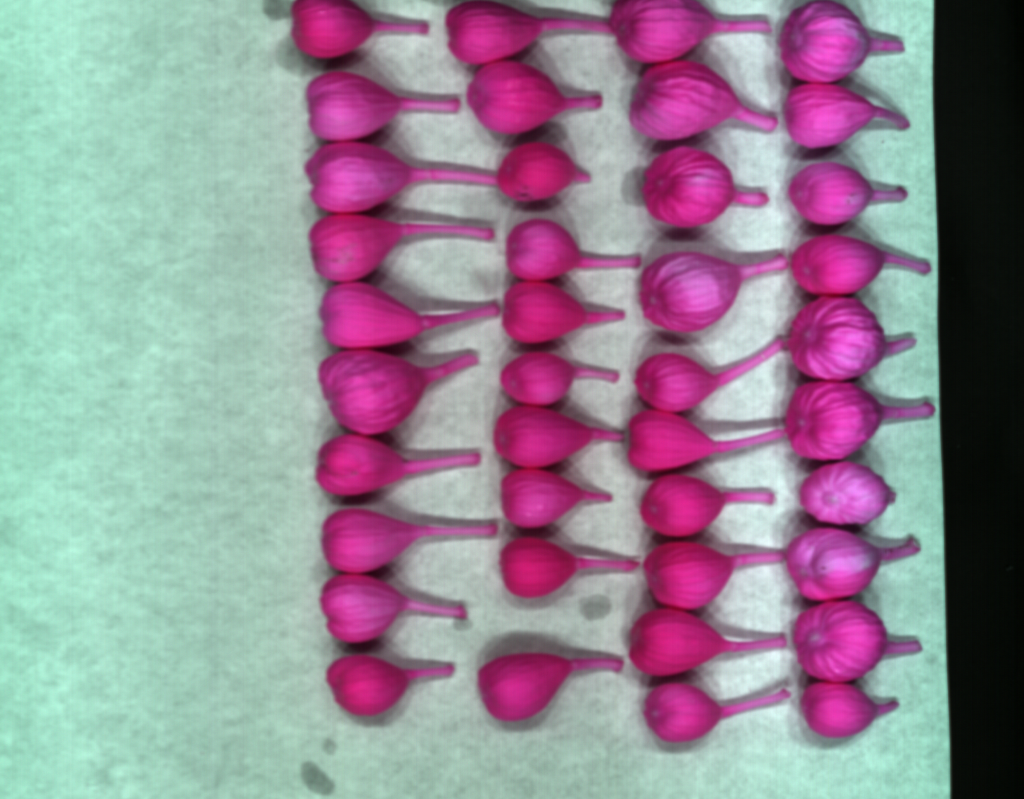
\includegraphics[width=6.0cm]{images/sample_figs_tray.png}}
\hspace{1mm}
\subfloat[\centering]{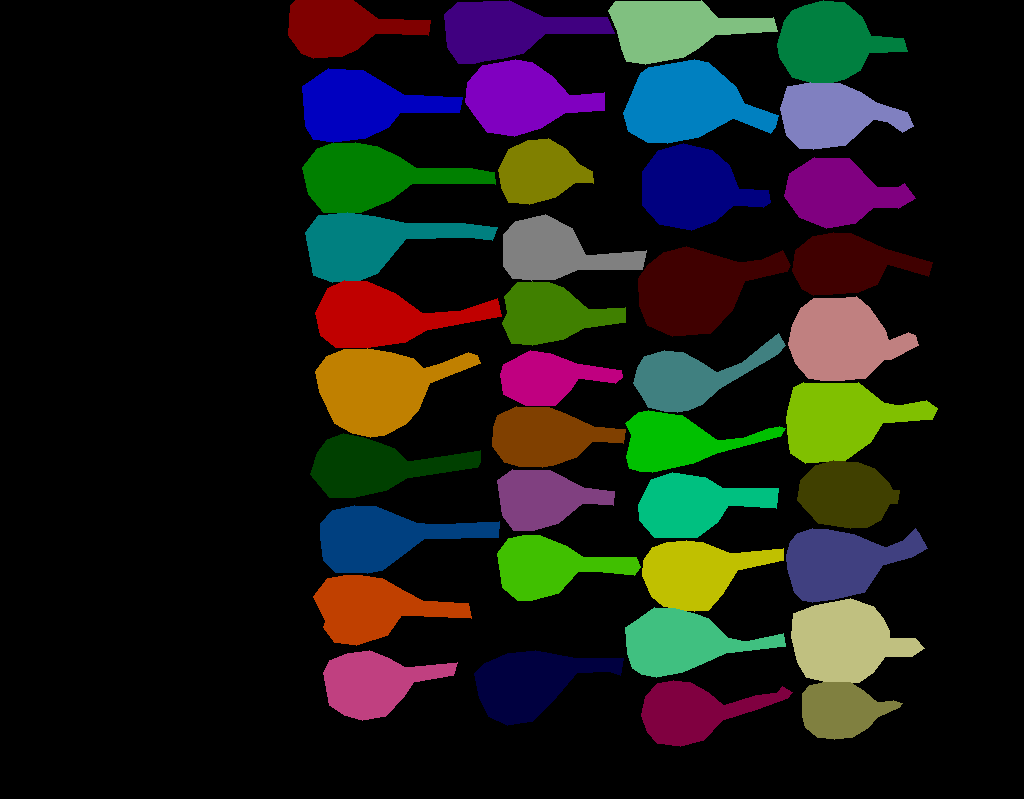
\includegraphics[width=6.0cm]{images/sample_figs_masks.png}}\\
\end{adjustwidth}
%} % If the paper is ``preprints'', please uncomment this parenthesis.
\caption{Figs tray before segmentation (\textbf{a}) and fig masks after segmentation (\textbf{b}).\label{fig2}}
\label{fig:1}
\end{figure}

Data processing and feature extraction were conducted using the Spectral Python (SPy) library. 
First, the header (.hdr) and binary (.raw) files were read to reconstruct the hyperspectral data cubes. 
Raw intensity values were then converted into relative reflectance through radiometric calibration, using the white and dark references acquired with each scene, according to equation \cite{morales_laboratory_2022}:

\begin{equation}
    R=\dfrac{I_{raw}-I_{dark}}{I_{white}-I_{dark}}
\end{equation}

%\[R=\dfrac{I_{raw}-I_{dark}}{I_{white}-I_{dark}}\]

where $I_{raw}$ is the raw image, $I_{dark}$ is the dark reference, and $I_{white}$ is the white reference. 
Following calibration, spectral features were extracted from the previously segmented ROIs. 
For each sample (fig), the mean and standard deviation of the reflectance were calculated across all spectral bands. 
These values were stored in two distinct feature matrices; one representing the average spectral signatures and the other capturing spectral variability, which served as inputs for the subsequent band selection stages.

\subsection{Dimensionality Reduction and Band Selection}

Although hyperspectral imagery provides abundant information, it suffers from significant redundancy due to the high correlation between contiguous spectral bands \cite{sawant_survey_2020}. 
This characteristic leads to the called \textit{curse of dimensionality} or Hughes phenomenon, where classification accuracy tends to decrease as the number of spectral bands increases, given a limited number of training samples \cite{hughes_mean_1968}. 
This high redundancy is shown in the figure \ref{fig:2} which is a correlation matrix of the spectral bands in the dataset generated of mean reflectance. 
The prominent structure formed in the diagonal of the matrix indicates groups of correlation coefficients near to 1.0. 
Furthermore, the high data volume significantly increases the computational burden required for processing. 
To address these challenges, band selection has proven to be an effective strategy for dimensionality reduction, eliminating redundancy while preserving the most discriminative spectral features \cite{sawant_survey_2020} \cite{nagasubramanian_hyperspectral_2018}. 
In this study, two metaheuristic approaches are employed for optimal band selection: Genetic Algorithms (GA) and Particle Swarm Optimization (PSO). 

\textcolor{red}{Comparing PSO and GA can provide valuable information to the problem at hand.  PSO is more effective in exploiting the search space by quickly adjusting solutions near the optimum, but it can get trapped in local optima due to its tendency to rapidly focus on specific areas. In contrast, GA favors global exploration and diversity, avoiding premature convergence and being more robust in multimodal spaces. Comparing both algorithms can help to identify whether the problem will require more exploration, where GA excels, or more exploitation, where PSO is more efficient. Not only will this improve the efficiency and robustness in the search for global optima, but it also can provide valuable insights to guide the next research steps.}

\begin{figure}[H]
%\isPreprints{\centering}{} % Only used for preprints
\centering
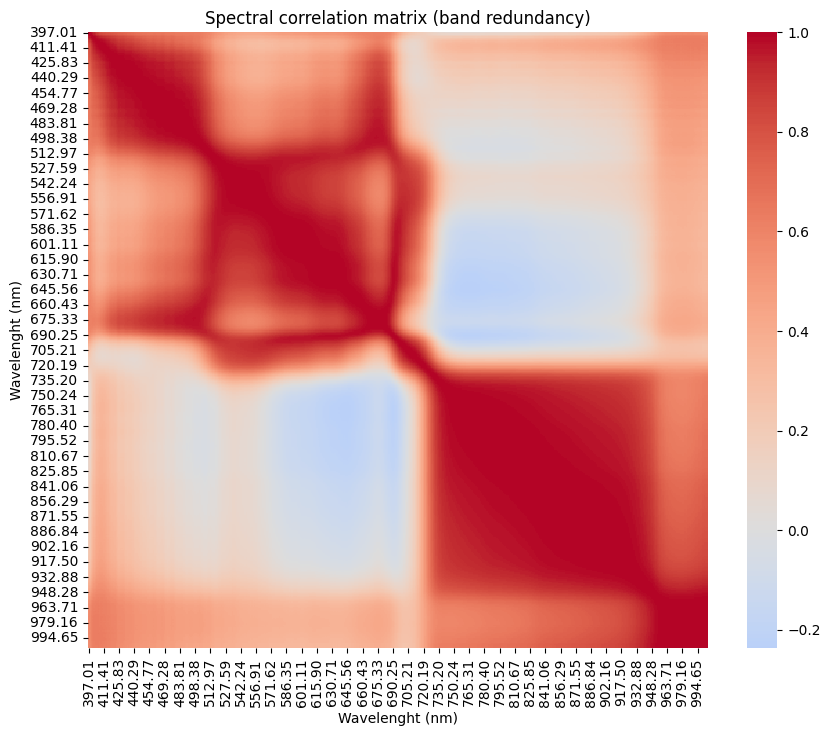
\includegraphics[width=10.0 cm]{images/spectral_colrrelation_matrix.png}
\caption{Figs mean values correlation matrix.}
\label{fig:2}
\end{figure}   
\unskip

\subsubsection{Feature Construction and Optimization Problem.}

To thoroughly capture the impact of fungal infection on both spectral response and surface texture, a concatenated feature vector was constructed combining the mean ($\mu$) and standard deviation ($\sigma$) of the reflectance values across all the pixels within the ROI for each spectral band. 
The mean reflectance characterizes the central tendency of the spectral signature \cite{nagasubramanian_hyperspectral_2018}, while the standard deviation quantifies the spatial variability of the sample surface \cite{hossain_color_2019}. 
Formally, for a hyperspectral image with $n$ bands, the complete pool of available features for the $i$-th sample is defined as $Xi=[\mu_i,1,\ldots \mu_i,n,\sigma_i,1,\ldots,\sigma_i,n]$. 
However, to maintain spectral consistency, the dimensionality reduction process was formulated as a band selection problem rather than an individual feature selection task. 
This means that selecting the $j$-th spectral band implies the simultaneous inclusion of both its corresponding mean ($\mu_j$) and standard deviation ($\sigma_j$) into the classifier input vector.

Therefore, the optimization search space consists of $n$ binary variables (where $n$ is the number of bands), but the dimensionality of the resulting feature vector sent to the classifier is $ 2\times{k} $, where $k$ is the number of selected bands. 
The objective is to find the binary vector $B=\{b1,\ldots,bn\}$ that maximizes the F1-Score \eqref{eq:f1_score}.

\begin{equation} \label{eq:f1_score}
    F1=2\times{\frac{Precision \times{Recall}}{Precision + Recall}}
\end{equation}

%\[ F1=2\times{\frac{Precision \times{Recall}}{Precision + Recall}} \]

The F1-Score was selected as the fitness function due to its ability to balance precision and recall. 
It is critical to penalize false negatives (infected figs misclassified as healthy), as these represent a significant health risk. 
Furthermore, the F1-Score provides a robust performance metric that effectively mitigates the bias potentially introduced by the slight class imbalance in the dataset.

\subsubsection{Genetic Algorithm}
The Genetic Algorithm (GA) is a metaheuristic optimization technique bio-inspired by natural evolution and genetic recombination. 
It encodes candidate solutions (individuals) as vectors and iteratively applies evolutionary operators such as selection, crossover, and mutation, often supplemented by elitism strategies \cite{eiben_introduction_2015}\cite{deb_multi-objective_2001}. 
\textcolor{red}{This implementation used a 448-bit binary string to encode the band subset, where a value of "1" indicates selection, and a "0" value denotes exclusion.}
%In the current implementation, a binary string of length 448 is used to encode the band subset; a value of '1' indicates selection, while '0' denotes exclusion. 
The algorithm evolves the population over successive generations to optimize the target fitness function. 
The specific parameter settings used in this study are detailed in Table \ref{tab1}.

\begin{table}[H] 
%\small % Change table font size
\caption{Genetic Algorithm parameters.\label{tab1}}
%\isPreprints{\centering}{} % Only used for preprints
\begin{tabularx}{\textwidth}{CCCCC}
\toprule
\textbf{Generations} & \textbf{\textcolor{red}{Population size}} & \textbf{Selection type} & \textbf{Crossover} & \textbf{Mutation rate}\\
\midrule
350 & 250 & Tournament of 2 & Single Point & 2.5\\
\bottomrule
\end{tabularx}
\noindent
\end{table}

\subsubsection{Particle Swarm Optimization Algorithm}
Particle Swarm Optimization (PSO) is a stochastic metaheuristic inspired by the collective social behavior of bird flocks and fish schools. 
Unlike traditional evolutionary algorithms that rely on recombination or crossover operators, PSO models the population members as particles traversing an n-dimensional search space. \textcolor{red}{By analogy, a swarm is similar to a population and a particle is similar to an individual.}   
Each particle is characterized by its current position (representing a candidate solution for the band selection) and a velocity vector that governs its trajectory. 
The movement of a particle is determined by updating its velocity based on a weighted sum of three distinct components \textcolor{red}{(inertia, cognitive and social)} \cite{eiben_introduction_2015}.

To enhance convergence efficiency and mitigate premature convergence to local optima, Time-Varying Acceleration Coefficients (TVAC) were implemented. \textcolor{red}{The inertia component was set at a fixed value.}
The cognitive coefficient ($C1$) was linearly decremented to encourage exploration during the early stages, while the social coefficient ($C2$) was linearly incremented to promote global exploitation towards the end of the search process. 
The dynamic adjustment of these parameters follows standard literature recommendations for high-dimensional optimization \cite{ratnaweera_self-organizing_2004}. 

\begin{equation}
    c_1(t)=(c_{1,f}-c_{1,i}) \frac{t}{T_{max}}+C_{1,i}
\end{equation}

\begin{equation}
    c_2(t)=(c_{2,f}-c_{2,i}) \frac{t}{T_{max}}+C_{2,i}
\end{equation}

%\[ c_1(t)=(c_{1,f}-c_{1,i}) \frac{t}{T_{max}}+C_{1,i} \]

%\[ c_2(t)=(c_{2,f}-c_{2,i}) \frac{t}{T_{max}}+C_{2,i} \]

Where:
\begin{itemize}
    \item $t$: Current iteration.
    \item $T_{max}$: Maximum number of iterations.
    \item $C_{1,i}$,$C_{2,i}$: Coefficient initial values.
    \item $C_{1,f}$,$C_{2,f}$: Coefficient final values.
\end{itemize}

The specific parameter settings used in this study are detailed in Table \ref{tab2}:
\begin{table}[H] 
%\small % Change table font size
\caption{PSO parameters.\label{tab2}}
%\isPreprints{\centering}{} % Only used for preprints
\begin{tabularx}{\textwidth}{CCCCCC}
\toprule
\textbf{Iterations} & \textbf{Particles} & \textbf{Cognitive coefficient (C1)} & \textbf{Social coefficient (C2)} & \textbf{Inertia} & \textbf{Mutation rate}\\
\midrule
650 & 200 & 0.4 to 2.5 & 2.5 to 0.4 & 0.7 & 0.2\\
\bottomrule
\end{tabularx}
\noindent
\end{table}

\subsection{Classification Model Implementation}
A Support Vector Machine (SVM) was implemented for the supervised classification task, selected for its proven robustness in high-dimensional spaces and effectiveness with limited datasets \cite{nagasubramanian_hyperspectral_2018}\cite{musci_ice_2020}. 
Given the non-linear nature of the spectral boundaries between healthy and infected samples, the Radial Basis Function (RBF) kernel was employed.

\subsubsection{Computational Strategy}
To mitigate the high computational overhead inherent to the iterative metaheuristic process (GA and PSO), a two stage evaluation strategy was implemented:

\begin{enumerate}
    \item Fast evaluator: A lightweight SVM configuration used as the wrapper within the fitness function. Its primary goal is to rapidly estimate how well perform the selected bands to guide the search algorithm, prioritizing the execution speed over hyperparameter tuning.
    \item Exhaustive evaluator: Upon completion of the optimization, the optimal band subset identified is used to train a rigorous final model, fine tuned via exhaustive hyperparameter search to maximize predictive performance.
\end{enumerate}

Before training, data normalization, using StandardScaler, was applied to ensure that both feature types (mean reflectance and standard deviation) contribute equally to the distance calculation. 
Finally, to ensure an unbiased evaluation, the winning model is evaluated on a test set that remained unseen during the optimization phase. 
The configuration parameters for both implementations are detailed in Table \ref{tab3}.

\begin{table}[H] 
%\small % Change table font size
\caption{SVM Parameters.\label{tab3}}
%\isPreprints{\centering}{} % Only used for preprints
\begin{tabularx}{\textwidth}{CCCCC}
\toprule
\textbf{Implementation} & \textbf{Kernel} & \textbf{Regularization ($C$)} & \textbf{Gamma ($\gamma$)} & \textbf{Validation method}\\
\midrule
Fast evaluator       & RBF & Fixed 1.0             & Fixed scale & k-fold CV ($k=3$)\\ \\
Exhaustive evaluator & RBF & Grid search 0.1 to 1000 & Grid search 0.001 to 1 & k-fold CV ($k=5$)\\
\bottomrule
\end{tabularx}
\noindent
\end{table}


%%%%%%%%%%%%%%%%%%%%%%%%%%%%%%%%%%%%%%%%%%
\section{Results}
\subsection{Spectral Characterization of Samples}
Figure \ref{fig:3}a displays the average spectral signatures relative to the healthy and infected fig samples across the full acquired spectral range (400--1000 nm). 
The shaded regions represent the standard deviation, illustrating the spectral variability within each class. 
As observed, the spectral patterns of both classes are visually similar, particularly in the visible region (400--700 nm). 
However, slight differences in reflectance intensity become more apparent in the Near Infrared (NIR) region (700--1000 nm), likely due to the structural degradation of the fig tissue caused by fungal colonization. 
This high spectral overlap confirms the complexity of the classification task. 
However, a different pattern is observed when analyzing the reflectance standard deviation. 
Figure \ref{fig:3}b presents the standard deviation per wavelength for both classes. 
It is observed that infected samples have a major variability compared to the healthy ones. 
This visual evidence leads to support the premise that the fungal infection affects the textural heterogeneity on the fig skin. 

\begin{figure}[H]
%\isPreprints{}{% This command is only used for ``preprints''.
\begin{adjustwidth}{0cm}{0cm}
\centering
%} % If the paper is ``preprints'', please uncomment this parenthesis.
\subfloat[\centering]{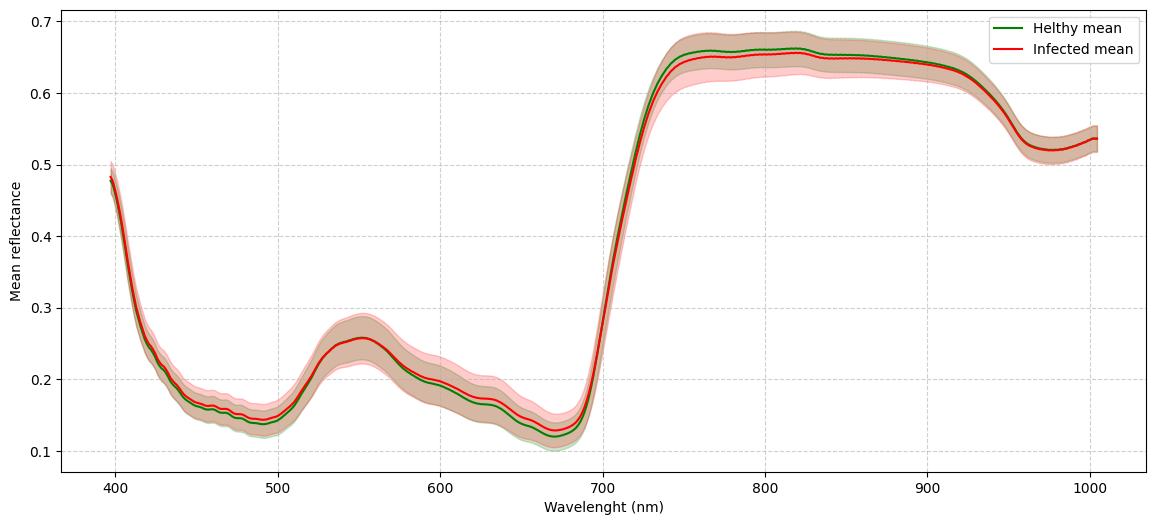
\includegraphics[width=13.0cm]{images/spectral_signature_mean_reflectance.png}}\\
\subfloat[\centering]{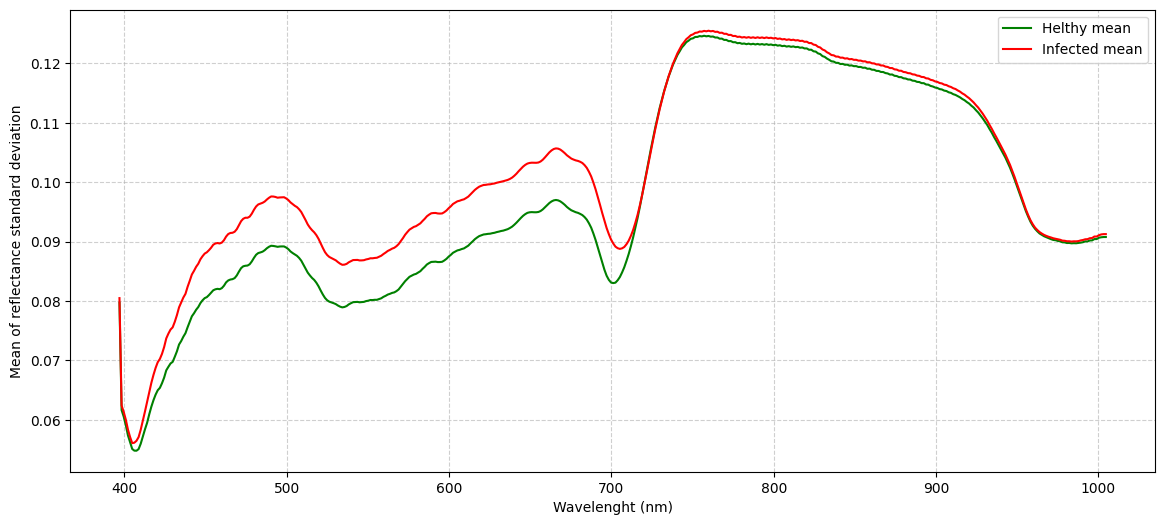
\includegraphics[width=13.0cm]{images/spectral_signature_mean_standard_deviation.png}}
%\hfill
%\isPreprints{}{% This command is only used for ``preprints''.
\end{adjustwidth}
%} % If the paper is ``preprints'', please uncomment this parenthesis.
\caption{Spectral characterization of the fig samples. (\textbf{a}) Average reflectance signatures showing the central tendency of healthy vs. infected classes. (\textbf{b}) Standard deviation signatures representing the spatial variability of the samples.\label{fig:3}}
\end{figure} 

\subsection{Impact of Feature Construction}
To validate the contribution of the standard deviation to the fungal classification, the band selection process was executed under two distinct feature configurations. 
Initially, the optimization was performed using only the mean reflectance per band, followed by a second scenario utilizing the combined mean and standard deviation vector. 
The optimization was conducted for target subset sizes of $k\in\{3,5,6\}$ over 30 independent runs. 
Table \ref{tab4} compares the average F1-Score obtained by the GA across both configurations.

\begin{table}[H] 
%\small % Change table font size
\caption{GA performance comparison (average F1-Score) between feature configurations.\label{tab4}}
%\isPreprints{\centering}{} % Only used for preprints
\begin{tabularx}{\textwidth}{CCCC}
\toprule
\textbf{Individual size} & \textbf{Mean reflectance only ($\mu$)} & \textbf{Combined features ($\mu + \sigma$)} & \textbf{Improvement (\%)} \\
\midrule
3 Bands & 0.663 & 0.755 & +9.2\% \\
5 Bands & 0.698 & 0.77  & +7.2\% \\
6 Bands & 0.721 & 0.773 & +5.2\%  \\
\bottomrule
\end{tabularx}
\noindent
\end{table}
%\begin{table}[H] 
%\caption{PSO performance comparison (average F1-Score) between feature configurations.\label{tab5}}
%\begin{tabularx}{\textwidth}{CCCC}
%\toprule
%\textbf{Individual size} & \textbf{Mean reflectance only ($\mu$)} & \textbf{Combined features ($\mu + \sigma$)} & \textbf{Improvement (\%)} \\
%\midrule
%3 Bands & 0.65 & 0.756 & +10.6\% \\
%5 Bands & 0.697 & 0.7  & +0.3\% \\
%6 Bands & 0.748 & 0.765 & +1.7\%  \\
%\bottomrule
%\end{tabularx}
%\noindent
%\end{table}
In addition to the previous performance metrics, the evolutionary behavior of the optimization process was analyzed. 
Figure \ref{fig:4} illustrates the average convergence history over 30 independent runs for both feature configurations. 
The solid lines represent the mean best fitness value at each generation, while the shaded regions indicate the standard deviation across runs.

\begin{figure}[H]
%\begin{adjustwidth}{-\extralength}{0cm}
\centering
\subfloat[\centering]{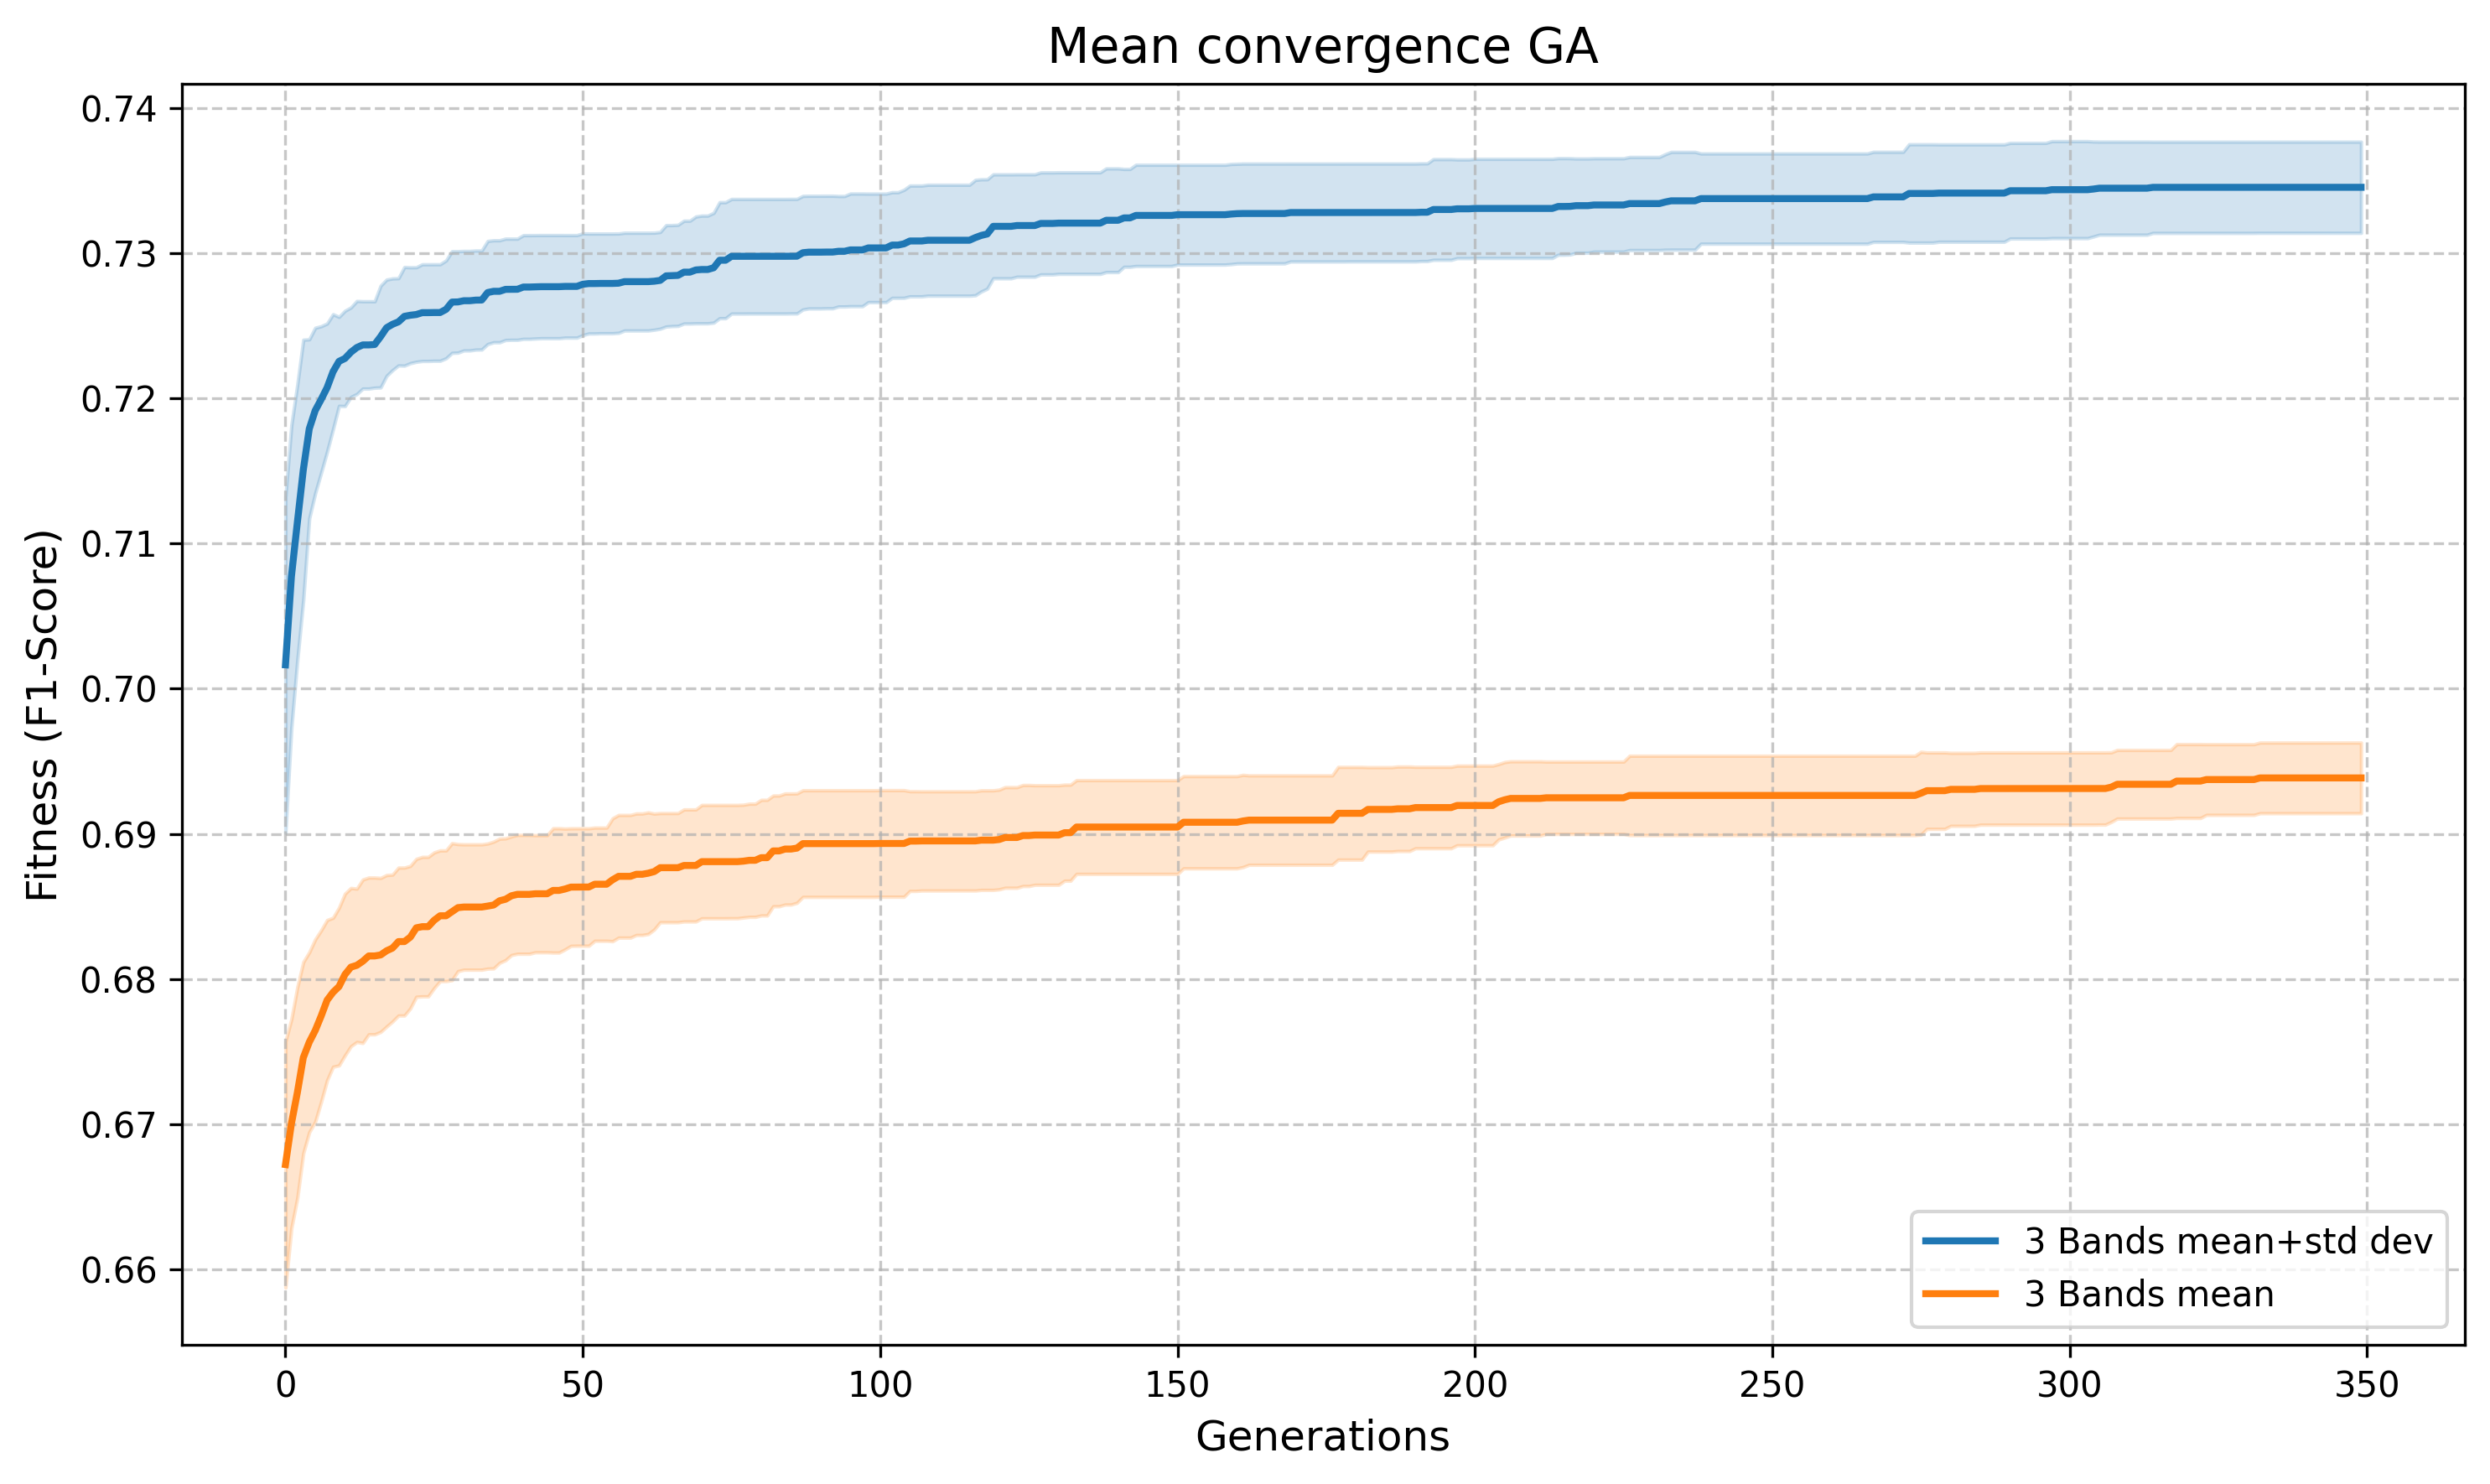
\includegraphics[width=7.2cm]{images/mean_convergence_3b.png}} 
%\hfill
\subfloat[\centering]{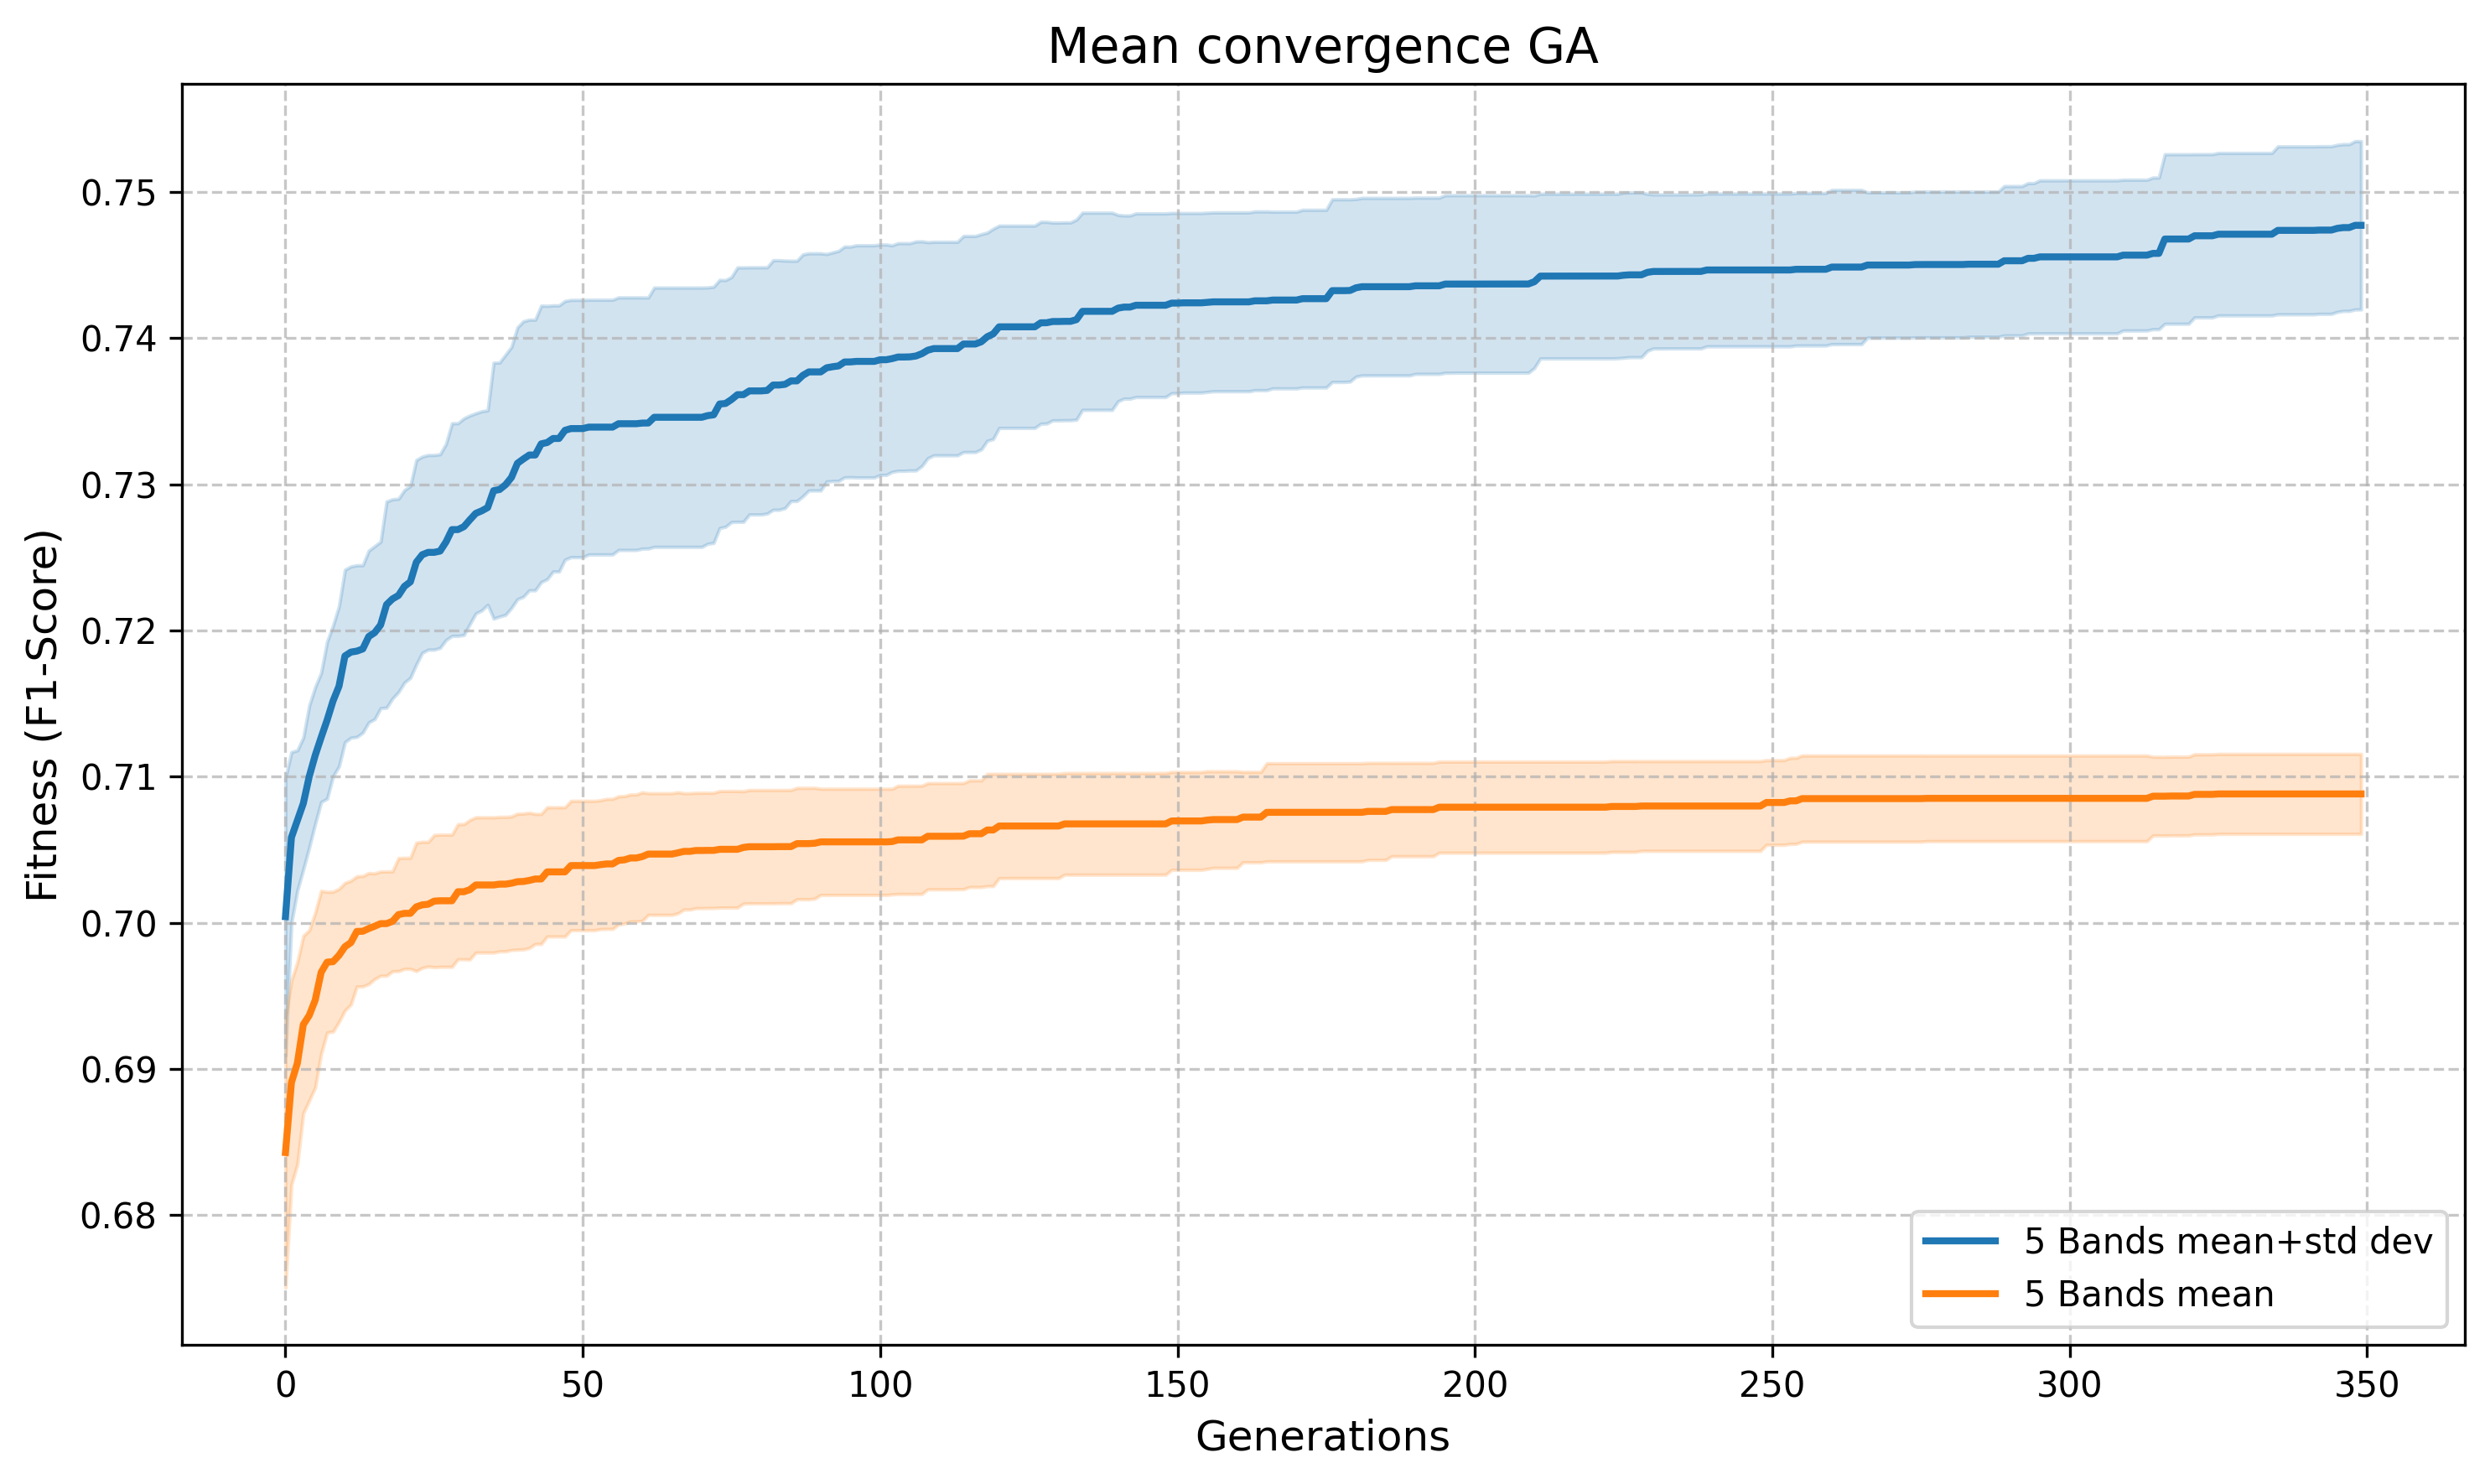
\includegraphics[width=7.2cm]{images/mean_convergence_5b.png}}\\
\subfloat[\centering]{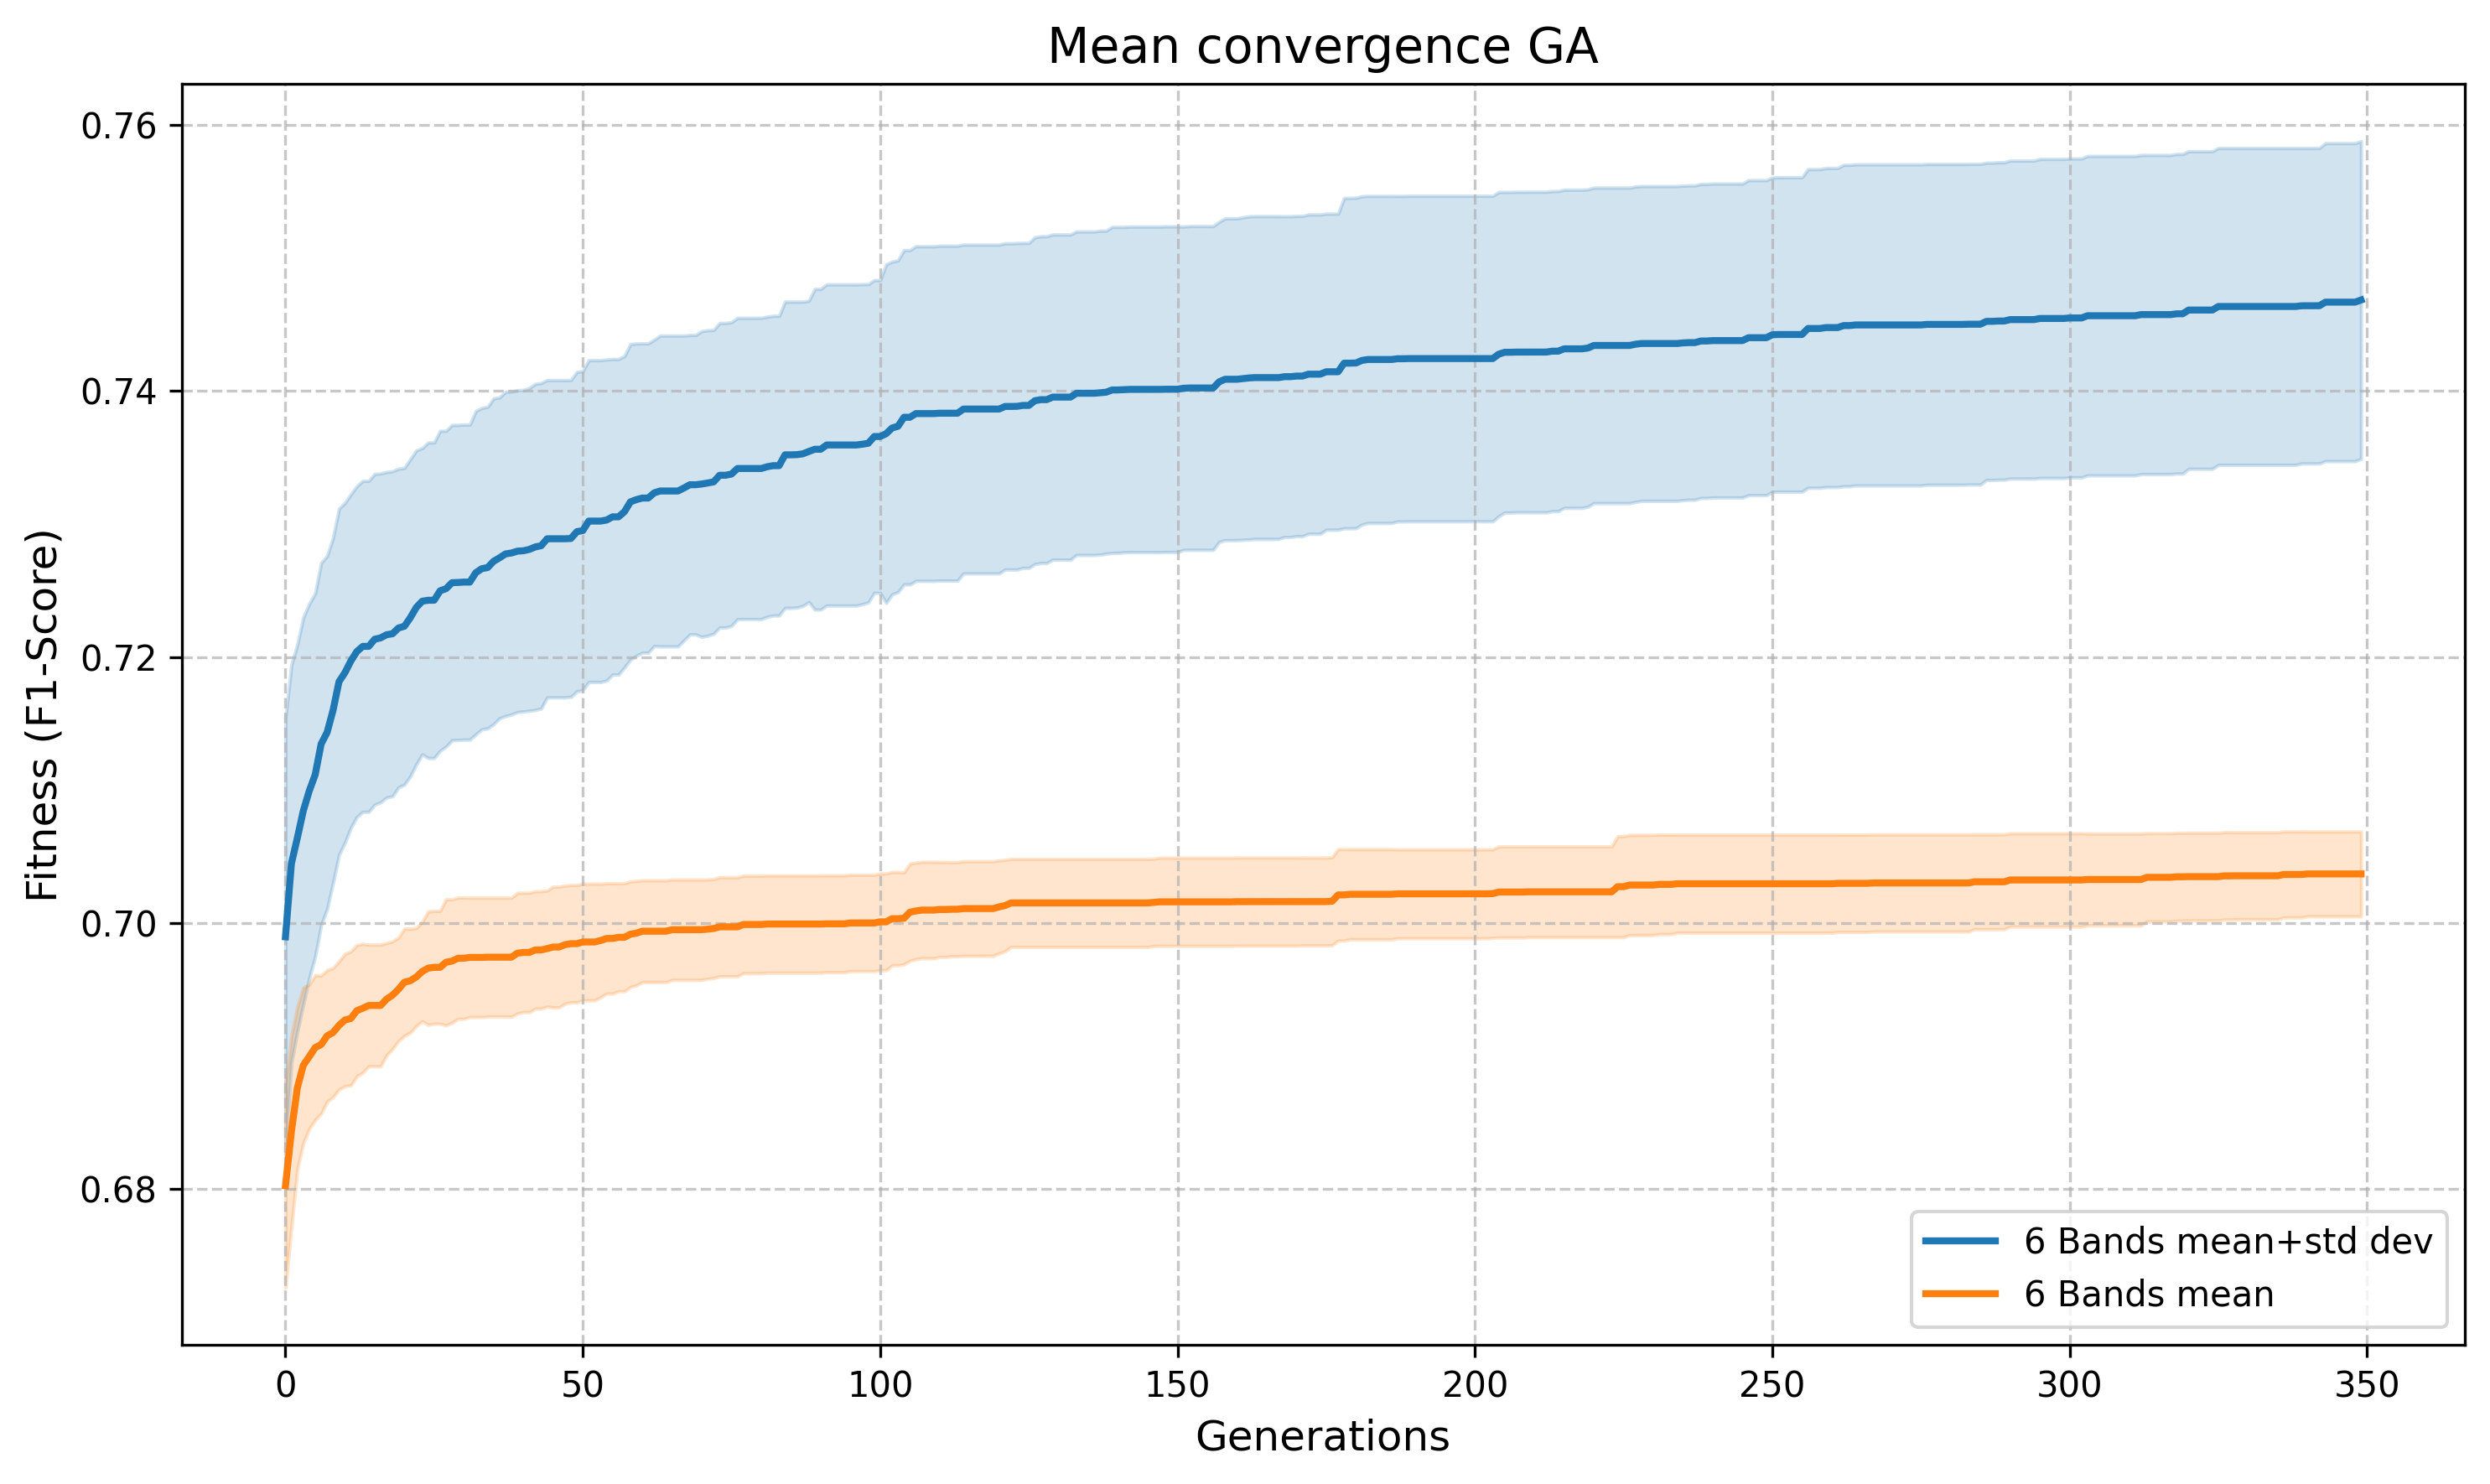
\includegraphics[width=7.2cm]{images/mean_convergence_6b.png}}
\hfill
%\end{adjustwidth}
%\caption{Convergence history of the Genetic Algorithm over 30 independent runs. (\textbf{a}) 3 bands optimization. (\textbf{b}) 5 bands optimization. (\textbf{c}) 6 bands optimization.\label{fig:4}}
\caption{Genetic Algorithm convergence profiles across 30 independent runs for: (\textbf{a}) 3-band; (\textbf{b}) 5-band; and (\textbf{c}) 6-band optimization scenarios.\label{fig:4}}
\end{figure} 

It can be observed that the Combined Features ($\mu+\sigma$) strategy (represented by the blue line) not only starts with a higher initial fitness but also maintains a superior trajectory throughout the generations compared to the Mean Reflectance Only approach. 
This convergence gap visually confirms that the additional textural information provides a more robust search space, allowing the proposed algorithm to find higher quality solutions more efficiently.

\subsection{Comparative Analysis of Metaheuristic Algorithms}
After the validation of the feature construction, the study focused on comparing the optimization capabilities of the GA versus PSO. 
To ensure statistical robustness, both algorithms were executed 30 times for each target subset size ($k\in\{3,5,6\}$) using the combined feature vector.

The figure \ref{fig:5} presents the boxplots summarizing the distribution of the F1-Scores obtained. 
The analysis reveals that the GA has a marginal difference with PSO in the context of hyperspectral band selection. 
Specifically, GA exhibited a higher median F1-Score when $k=\{5, 6\}$ subset sizes, particularly in the most scenario (k=6), where it achieved a median value of 0.773. 
However, PSO had a slight advantage in the 3 bands scenario. 
Furthermore, the interquartile ranges for GA were consistently narrower compared to PSO, indicating superior algorithmic stability and reproducibility.

\begin{figure}[H]
\centering
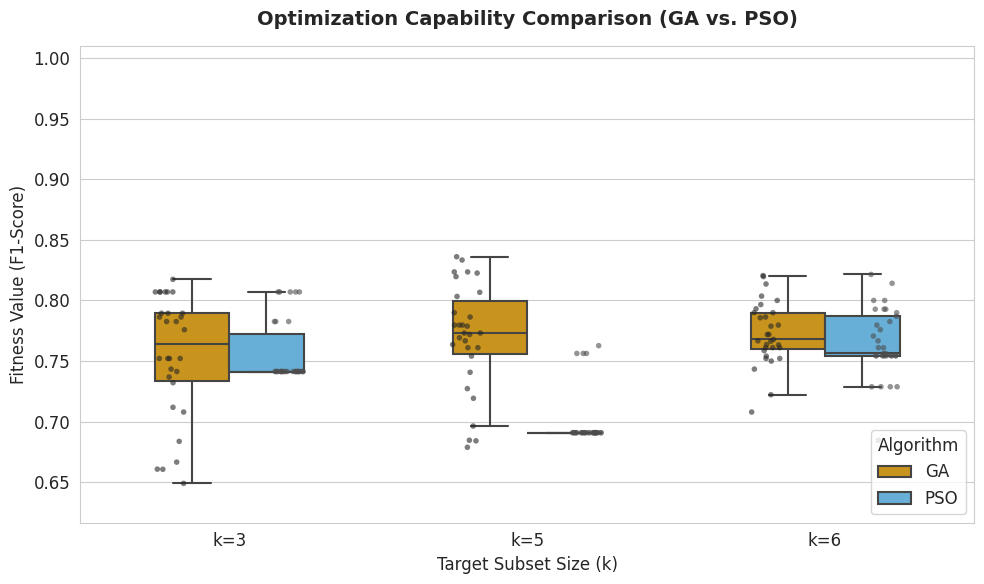
\includegraphics[width=11.0 cm]{images/boxplot_comparison_mean_std.png}
\caption{Boxplot comparison GA vs. PSO with ($\mu+\sigma$) features.}
\label{fig:5}
\end{figure}   
\unskip
\hfill \break

Notably, the absolute maximum F1-Score of the entire study (0.836) was achieved by PSO using the 5-band subset with the ($\mu+\sigma$) configuration. 
However, it is noteworthy that the configuration using only the mean ($\mu$) with 6 bands yielded a nearly identical score of 0.832. 
This suggests that the inclusion of the standard deviation stabilizes the search process and improves classification performance when the feature subset is small (e.g., 3 bands); however, this advantage diminishes as more bands are added. 
Figure \ref{fig:6} illustrates this phenomenon, showing how the variance in the solution space increases for the 6-band configuration that relies solely on the mean.

\begin{figure}[H]
\centering
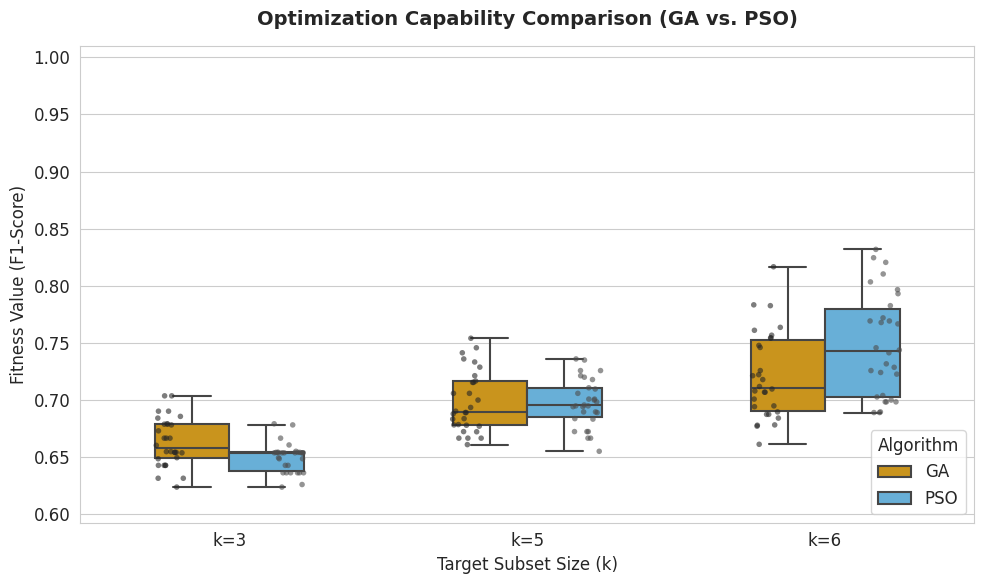
\includegraphics[width=11.0 cm]{images/boxplot_comparison_mean.png}
\caption{Boxplot comparison GA vs. PSO only with ($\mu$) feature.}
\label{fig:5}
\end{figure}   
\unskip

%%%%%%%%%%%%%%%%%%%%%%%%%%%%%%%%%%%%%%%%%%
\section{Discussion}
\subsection{Physical interpretation}
% TODO
The spatial distribution of the selected bands in the best individuals was analyzed against the spectral signatures of the samples. 
Figure \ref{fig:6} illustrates the mean reflectance spectra for healthy (green) and infected (red) figs, with the vertical blue dashed lines representing the bands of the best individuals selected by the GA across the 30 execution runs for $K\in\{3, 5, 6\}$.

The visualization reveals a not uniform distribution of selected bands; the bands cluster in three different spectral regions that correspond to known physiological changes caused by plant diseases.

\begin{enumerate}
    \item 400 -- 450 nm: A cluster of bands is observed in the lower visible spectrum. This region is associated with the absorption of pigments such as carotenoids and anthocyanins \cite{mahlein_plant_2016}.
    \item 700 -- 750 nm: This accumulation of selected bands around the red edge (between visible red and near infra red) is sensitive to stress induced changes in cellular structure \cite{mahlein_plant_2016}. 
    \item  950 - 1000 nm: The selected bands in the end of the selected spectrum coincides with second overtone of the O-H bond stretch, indicating possible signs of dehydration \cite{nicolai_nondestructive_2007}.
\end{enumerate}

\begin{figure}[H]
\centering
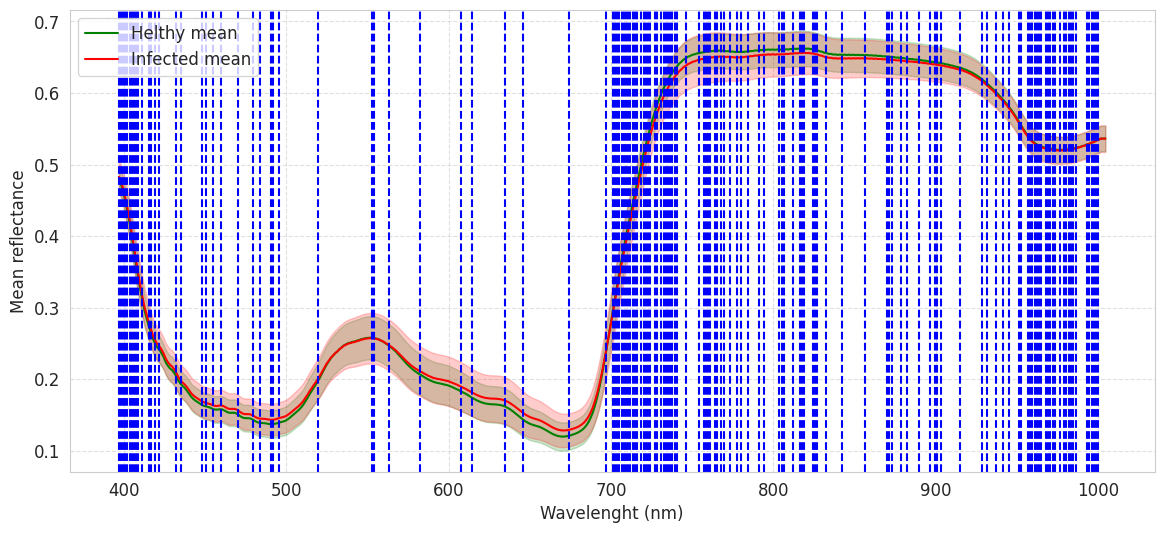
\includegraphics[width=13.0 cm]{images/spectral_signature_selected_bands_ga.png}
\caption{Mean reflectance spectral signature with vertical lines indicating the selected bands by the best individuals of the GA.}
\label{fig:6}
\end{figure}   
\unskip

\subsection{Conclusions and Future Work}
This study presented a non invasive methodology for the detection of \textit{Aspergillus flavus} in figs using hyperspectral imaging coupled with metaheuristic band selection. 
By constructing a statistical feature vector based on the spectral mean ($\mu$) and standard deviation ($\sigma$), the proposed approach successfully reduced the high dimensional hyperspectral data into a compact subset of informative variables.

\subsubsection{Key findings}
\begin{enumerate}
    \item Algorithmic Performance: In the majority of cases, the GA exhibited slightly better average performance compared to PSO. However, PSO identified the global maximum, the absolute best solution. This indicates that both metaheuristics possess comparable optimization capabilities for this spectral selection task.
    \item Feature relevance: The results highlighted that, on average, the inclusion of the standard deviation ($\mu+\sigma$) significantly improved performance in lower dimensional subsets ($k\in\{3,5\}$). However, as the number of selected bands increases, this performance gain becomes marginal, suggesting that the added complexity of the standard deviation is less critical when more spectral information is available.
    \item Physical Consistency: The spectral bands selected correspond with relevant biological regions; they are aligned with the visible pigmentation changes and NIR water content regions. 
\end{enumerate}

\subsubsection{Future work.}
Having the current results in mind several paths for future work have been identified to further enhance the system performance:

\begin{itemize}
    \item Multi-Objective Optimization: Instead of constrain the search to a fixed or arbitrary number of bands, as done in the present work, future iterations might employ multi-objective optimization algorithms. The goal is to maximize the F1-Score and minimize the number of bands, thereby finding the optimal Pareto front that balances classification accuracy with system simplicity.
    \item Advanced Classifiers: While the SVM classifier used demonstrated solid performance, we aim to explore more other machine learning algorithms such as Random Forest and XGBoost, which may offer better handling of the non linear interactions of the spectral data. 
    \item Co-evolutionary Strategies: To improve the feature selection process itself, we propose exploring co-evolutionary techniques. These methods could allow the population of solutions (bands) and the population of strategies (classifier parameters) to evolve together, potentially discovering more effective spectral combinations that a standard evolutionary approach might miss.
\end{itemize}

%%%%%%%%%%%%%%%%%%%%%%%%%%%%%%%%%%%%%%%%%%
\vspace{6pt} 

%%%%%%%%%%%%%%%%%%%%%%%%%%%%%%%%%%%%%%%%%%
%% optional
%\supplementary{The following supporting information can be downloaded at:  \linksupplementary{s1}, Figure S1: title; Table S1: title; Video S1: title.}

% Only for journal Methods and Protocols:
% If you wish to submit a video article, please do so with any other supplementary material.
% \supplementary{The following supporting information can be downloaded at: \linksupplementary{s1}, Figure S1: title; Table S1: title; Video S1: title. A supporting video article is available at doi: link.}

% Only used for preprtints:
% \supplementary{The following supporting information can be downloaded at the website of this paper posted on \href{https://www.preprints.org/}{Preprints.org}.}

% Only for journal Hardware:
% If you wish to submit a video article, please do so with any other supplementary material.
% \supplementary{The following supporting information can be downloaded at: \linksupplementary{s1}, Figure S1: title; Table S1: title; Video S1: title.\vspace{6pt}\\
%\begin{tabularx}{\textwidth}{lll}
%\toprule
%\textbf{Name} & \textbf{Type} & \textbf{Description} \\
%\midrule
%S1 & Python script (.py) & Script of python source code used in XX \\
%S2 & Text (.txt) & Script of modelling code used to make Figure X \\
%S3 & Text (.txt) & Raw data from experiment X \\
%S4 & Video (.mp4) & Video demonstrating the hardware in use \\
%... & ... & ... \\
%\bottomrule
%\end{tabularx}
%}

%%%%%%%%%%%%%%%%%%%%%%%%%%%%%%%%%%%%%%%%%%
%\authorcontributions{For research articles with several authors, a short paragraph specifying their individual contributions must be provided. The following statements should be used ``Conceptualization, X.X. and Y.Y.; methodology, X.X.; software, X.X.; validation, X.X., Y.Y. and Z.Z.; formal analysis, X.X.; investigation, X.X.; resources, X.X.; data curation, X.X.; writing---original draft preparation, X.X.; writing---review and editing, X.X.; visualization, X.X.; supervision, X.X.; project administration, X.X.; funding acquisition, Y.Y. All authors have read and agreed to the published version of the manuscript.'', please turn to the  \href{http://img.mdpi.org/data/contributor-role-instruction.pdf}{CRediT taxonomy} for the term explanation. Authorship must be limited to those who have contributed substantially to the work~reported.}

\funding{This research received no external funding.}

%\institutionalreview{In this section, you should add the Institutional Review Board Statement and approval number, if relevant to your study. You might choose to exclude this statement if the study did not require ethical approval. Please note that the Editorial Office might ask you for further information. Please add “The study was conducted in accordance with the Declaration of Helsinki, and approved by the Institutional Review Board (or Ethics Committee) of NAME OF INSTITUTE (protocol code XXX and date of approval).” for studies involving humans. OR “The animal study protocol was approved by the Institutional Review Board (or Ethics Committee) of NAME OF INSTITUTE (protocol code XXX and date of approval).” for studies involving animals. OR “Ethical review and approval were waived for this study due to REASON (please provide a detailed justification).” OR “Not applicable” for studies not involving humans or animals.}

%\informedconsent{Any research article describing a study involving humans should contain this statement. Please add ``Informed consent was obtained from all subjects involved in the study.'' OR ``Patient consent was waived due to REASON (please provide a detailed justification).'' OR ``Not applicable'' for studies not involving humans. You might also choose to exclude this statement if the study did not involve humans.

%Written informed consent for publication must be obtained from participating patients who can be identified (including by the patients themselves). Please state ``Written informed consent has been obtained from the patient(s) to publish this paper'' if applicable.}


%\dataavailability{We encourage all authors of articles published in MDPI journals to share their research data. In this section, please provide details regarding where data supporting reported results can be found, including links to publicly archived datasets analyzed or generated during the study. Where no new data were created, or where data is unavailable due to privacy or ethical restrictions, a statement is still required. Suggested Data Availability Statements are available in section ``MDPI Research Data Policies'' at \url{https://www.mdpi.com/ethics}.} 

% Only for journal Drones
%\durcstatement{Current research is limited to the [please insert a specific academic field, e.g., XXX], which is beneficial [share benefits and/or primary use] and does not pose a threat to public health or national security. Authors acknowledge the dual-use potential of the research involving xxx and confirm that all necessary precautions have been taken to prevent potential misuse. As an ethical responsibility, authors strictly adhere to relevant national and international laws about DURC. Authors advocate for responsible deployment, ethical considerations, regulatory compliance, and transparent reporting to mitigate misuse risks and foster beneficial outcomes.}

% Only for journal Nursing Reports
%\publicinvolvement{Please describe how the public (patients, consumers, carers) were involved in the research. Consider reporting against the GRIPP2 (Guidance for Reporting Involvement of Patients and the Public) checklist. If the public were not involved in any aspect of the research add: ``No public involvement in any aspect of this research''.}
%
%% Only for journal Nursing Reports
%\guidelinesstandards{Please add a statement indicating which reporting guideline was used when drafting the report. For example, ``This manuscript was drafted against the XXX (the full name of reporting guidelines and citation) for XXX (type of research) research''. A complete list of reporting guidelines can be accessed via the equator network: \url{https://www.equator-network.org/}.}
%
%% Only for journal Nursing Reports
%\useofartificialintelligence{Please describe in detail any and all uses of artificial intelligence (AI) or AI-assisted tools used in the preparation of the manuscript. This may include, but is not limited to, language translation, language editing and grammar, or generating text. Alternatively, please state that “AI or AI-assisted tools were not used in drafting any aspect of this manuscript”.}

\acknowledgments{his research is supported by Spanish Ministry of Science and Innovation under project PID2023-147409NB-C22 funded by MCIN-/AEI-/10.130-39/501100011033, Junta de Extremadura, project GR24142 and by “ERDF A way of making Europe”}

\conflictsofinterest{Declare conflicts of interest or state ``The authors declare no conflicts of interest.'' Authors must identify and declare any personal circumstances or interest that may be perceived as inappropriately influencing the representation or interpretation of reported research results. Any role of the funders in the design of the study; in the collection, analyses or interpretation of data; in the writing of the manuscript; or in the decision to publish the results must be declared in this section. If there is no role, please state ``The funders had no role in the design of the study; in the collection, analyses, or interpretation of data; in the writing of the manuscript; or in the decision to publish the results''.} 

%%%%%%%%%%%%%%%%%%%%%%%%%%%%%%%%%%%%%%%%%%
%% Optional

%% Only for journal Encyclopedia
%\entrylink{The Link to this entry published on the encyclopedia platform.}

\abbreviations{Abbreviations}{
The following abbreviations are used in this manuscript:
\\

\noindent 
\begin{tabular}{@{}ll}
GA & Genetic Algorithm\\
HSI & Hyperspectral Imaging\\
PSO & Particle Swarm Optimization\\
SVM & Support Vector Machine\\
MDPI & Multidisciplinary Digital Publishing Institute\\
%DOAJ & Directory of open access journals\\
%TLA & Three letter acronym\\
%LD & Linear dichroism
\end{tabular}
}

%%%%%%%%%%%%%%%%%%%%%%%%%%%%%%%%%%%%%%%%%%%
%%% Optional
%\appendixtitles{no} % Leave argument "no" if all appendix headings stay EMPTY (then no dot is printed after "Appendix A"). If the appendix sections contain a heading then change the argument to "yes".
%\appendixstart
%\appendix
%\section[\appendixname~\thesection]{}
%\subsection[\appendixname~\thesubsection]{}
%The appendix is an optional section that can contain details and data supplemental to the main text---for example, explanations of experimental details that would disrupt the flow of the main text but nonetheless remain crucial to understanding and reproducing the research shown; figures of replicates for experiments of which representative data are shown in the main text can be added here if brief, or as Supplementary Data. Mathematical proofs of results not central to the paper can be added as an appendix.
%
%\begin{table}[H] 
%\caption{This is a table caption.\label{tab5}}
%%\newcolumntype{C}{>{\centering\arraybackslash}X}
%\begin{tabularx}{\textwidth}{CCC}
%\toprule
%\textbf{Title 1}	& \textbf{Title 2}	& \textbf{Title 3}\\
%\midrule
%Entry 1		& Data			& Data\\
%Entry 2		& Data			& Data\\
%\bottomrule
%\end{tabularx}
%\end{table}
%
%\section[\appendixname~\thesection]{}
%All appendix sections must be cited in the main text. In the appendices, Figures, Tables, etc. should be labeled, starting with ``A''---e.g., Figure A1, Figure A2, etc.
%
%%%%%%%%%%%%%%%%%%%%%%%%%%%%%%%%%%%%%%%%%%%
%\isPreprints{}{% This command is only used for ``preprints''.
\begin{adjustwidth}{-\extralength}{0cm}
%} % If the paper is ``preprints'', please uncomment this parenthesis.
%\printendnotes[custom] % Un-comment to print a list of endnotes

\reftitle{References}

% Please provide either the correct journal abbreviation (e.g. according to the “List of Title Word Abbreviations” http://www.issn.org/services/online-services/access-to-the-ltwa/) or the full name of the journal.
% Citations and References in Supplementary files are permitted provided that they also appear in the reference list here. 

%=====================================
% References, variant A: external bibliography
%=====================================

\bibliography{refs}


% If authors have biography, please use the format below
%\section*{Short Biography of Authors}
%\bio
%{\raisebox{-0.35cm}{\includegraphics[width=3.5cm,height=5.3cm,clip,keepaspectratio]{Definitions/author1.pdf}}}
%{\textbf{Firstname Lastname} Biography of first author}
%
%\bio
%{\raisebox{-0.35cm}{\includegraphics[width=3.5cm,height=5.3cm,clip,keepaspectratio]{Definitions/author2.jpg}}}
%{\textbf{Firstname Lastname} Biography of second author}

% For the MDPI journals use author-date citation, please follow the formatting guidelines on http://www.mdpi.com/authors/references
% To cite two works by the same author: \citeauthor{ref-journal-1a} (\citeyear{ref-journal-1a}, \citeyear{ref-journal-1b}). This produces: Whittaker (1967, 1975)
% To cite two works by the same author with specific pages: \citeauthor{ref-journal-3a} (\citeyear{ref-journal-3a}, p. 328; \citeyear{ref-journal-3b}, p.475). This produces: Wong (1999, p. 328; 2000, p. 475)

%%%%%%%%%%%%%%%%%%%%%%%%%%%%%%%%%%%%%%%%%%
%% for journal Sci
%\reviewreports{\\
%Reviewer 1 comments and authors' response\\
%Reviewer 2 comments and authors' response\\
%Reviewer 3 comments and authors' response
%}
%%%%%%%%%%%%%%%%%%%%%%%%%%%%%%%%%%%%%%%%%%
\PublishersNote{}
%\isPreprints{}{% This command is only used for ``preprints''.
\end{adjustwidth}
%} % If the paper is ``preprints'', please uncomment this parenthesis.
\end{document}
